%------------------------------------------------------------------------------
% Beginning of journal.tex
%------------------------------------------------------------------------------
%
% AMS-LaTeX version 2 sample file for journals, based on amsart.cls.
%
%        ***     DO NOT USE THIS FILE AS A STARTER.      ***
%        ***  USE THE JOURNAL-SPECIFIC *.TEMPLATE FILE.  ***
%
% Replace amsart by the documentclass for the target journal, e.g., tran-l.
%
\documentclass{amsart}


\usepackage{algorithm}
\usepackage{algorithmic}
\usepackage{amssymb}
\usepackage{amsfonts}
\usepackage{xcolor}
\usepackage{graphicx}
\usepackage[backref]{hyperref}
\usepackage{cleveref}
\usepackage{diagbox}
\usepackage{subfigure}
\usepackage[switch]{lineno}

\newtheorem{theorem}{Theorem}[section]
\newtheorem{lemma}[theorem]{Lemma}
\newtheorem{corollary}[theorem]{Corollary}

\theoremstyle{definition}
\newtheorem{definition}[theorem]{Definition}
\newtheorem{example}[theorem]{Example}
\newtheorem{xca}[theorem]{Exercise}

\theoremstyle{remark}
\newtheorem{remark}[theorem]{Remark}

% \usepackage{amsthm}

\crefname{section}{section}{sections}
\crefname{subsection}{subsection}{subsections}
\Crefname{section}{Section}{Sections}
\Crefname{subsection}{Subsection}{Subsections}
\Crefname{figure}{Figure}{Figures}
\crefname{figure}{figure}{figures}
\crefname{lemma}{lemma}{lemmas}
\Crefname{lemma}{Lemma}{Lemmas}
\crefname{definition}{definition}{definitions}
\crefname{remark}{remark}{remarks}
\crefname{table}{table}{tables}

\numberwithin{equation}{section}

%    Absolute value notation
\newcommand{\abs}[1]{\lvert#1\rvert}

%    Blank box placeholder for figures (to avoid requiring any
%    particular graphics capabilities for printing this document).
\newcommand{\blankbox}[2]{%
  \parbox{\columnwidth}{\centering
%    Set fboxsep to 0 so that the actual size of the box will match the
%    given measurements more closely.
    \setlength{\fboxsep}{0pt}%
    \fbox{\raisebox{0pt}[#2]{\hspace{#1}}}%
  }%
}

\begin{document}

\title{Second-order  difference-quadrature approach    on graded meshes  for fractional Laplacian }

%    Information for first author

\author{Minghua Chen}
%    Address of record for the research reported here
\address{School of Mathematics and Statistics, Gansu Key Laboratory of Applied Mathematics and Complex Systems, Lanzhou University, Lanzhou 730000, P.R. China }
\email{chenmh@lzu.edu.cn}


\author{Jianxing Han}
\address{School of Mathematics and Statistics, Gansu Key Laboratory of Applied Mathematics and Complex Systems, Lanzhou University, Lanzhou 730000, P.R. China}
\email{hanjx2023@lzu.edu.cn}


\author{Natalia Kopteva}
\address{Department of Mathematics and Statistics
University of Limerick
Limerick, V94 T9PX, Ireland}
\email{	Natalia.Kopteva@ul.ie}
%\address{Department of Applied Physics and Applied Mathematics, Columbia University, New York, NY 10027}
%    Current address
%\curraddr{Department of Applied Physics and Applied Mathematics, Columbia University, New York, NY 10027}
%    \thanks will become a 1st page footnote.
%\thanks{The  author was partially supported by the China Scholarship Council (CSC)}
%\thanks{This work was supported by NSFC 11271173
%and NSF  DMS-1318586.}
  %  Information for second author
  

%\thanks{Support information for the  third author.}  

% \author{Martin Stynes}
% \address{Applied and Computational Mathematics Division, Beijing Computational Science Research
% Center, Beijing 100094,  P.R. China}
% \email{m.stynes@csrc.ac.cn}
%\thanks{Support information for the second author.}

  %  Information for third %author



%    General info
\subjclass[2010]{Primary 26A33, 26A30,  65L20.}
%
\keywords{Fractional Laplacian, Riesz fractional derivative, finite difference-quadrature method,  singular source term,  stability and convergence, graded meshes}


\begin{abstract}
This paper deals with the {\em integral-differential} version of the   fractional Laplacian   via the Riesz fractional derivative. The numerical analysis presents significant challenges,  partly because the solution to the problem has a weak singularity at the boundary, and the model equation  can involve a singular  source term. In such cases, many prevalent numerical methods may suffer from a severe order reduction. To fill in this gap, we combine  finite difference method and  numerical quadrature, called  difference-quadrature method,    to approximate  the  {\em differential} and    {\em integral}   operator of  the   fractional Laplacian  on graded meshes, respectively. We  design a grid mapping function and a natural-skew  ordering  to handle  local truncation errors, and construct an appropriate  right-preconditioner for the resulting matrix algebraic equation. By utilizing the H\"older regularity of the data, we prove that the proposed scheme  is  second-order convergence on graded meshes even if the source term is hypersingular. Numerical experiments illustrate the theoretical results.
\end{abstract}

\maketitle
\pagestyle{myheadings}
\thispagestyle{plain}
\markboth{M. H. CHEN, J. X. HAN}{Riesz Fractional Laplacian}
%\section*{This is an unnumbered first-level section head}
%This is an example of an unnumbered first-level heading.

%% The correct journal style for \specialsection is all uppercase; a known bug
%% in amsart.cls prevents this, so input must be uppercase until it is fixed.
%\specialsection*{This is a Special Section Head}
%\specialsection*{THIS IS A SPECIAL SECTION HEAD}
%This is an example of a special section head%
%%%%%%%%%%%%%%%%%%%%%%%%%%%%%%%%%%%%%%%%%%%%%%%%%%%%%%%%%%%%%%%%%%%%%%%%
%\footnote{Here is an example of a footnote. Notice that this footnote
%text is running on so that it can stand as an example of how a footnote
%with separate paragraphs should be written.
%\par
%And here is the beginning of the second paragraph.}%
%%%%%%%%%%%%%%%%%%%%%%%%%%%%%%%%%%%%%%%%%%%%%%%%%%%%%%%%%%%%%%%%%%%%%%%%




\linenumbers


% Chapter 1: Introduction
\section{Introduction}
Fractional Laplacian is a powerful tool in modeling phenomena for anomalous diffusion, which appears naturally in the \(\alpha\)-stable L\'evy process instead of the standard Brownian motion % DOI. 10.1137/22M1504706
\cite{ABBM2018,Bertoin:96,Getoor1961,MR2584076, MK:00}. It can be found in many applications, such as 
% turbulence [22], 
porous media flow \cite{MR2737788},
image processing \cite{MR3394445}, 
biophysics \cite{Andreu:10}.
In this work, we study a second-order difference-quadrature scheme on graded meshes for the integral-differential version of the   fractional Laplacian  
\begin{equation} \label{eq:equation}
  \begin{cases}
    (-\Delta)^{\frac{\alpha}{2}} u(x) = f(x) & x \in \Omega,                    \\
    u(x) = 0                                 & x \in \mathbb{R} \setminus \Omega.
  \end{cases}
\end{equation}
Here  $(-\Delta)^{\frac{\alpha}{2}}$ is the integral-differential   fractional Laplacian, in terms of the Riesz (left and right Riemann-Liouville) fractional derivative \cite{ABBM2018, HuangO:14, MR4043885,MR2796453}, defined by  
\begin{equation} \label{def:operator}
  \begin{split}  
      (-\Delta)^{\frac{\alpha}{2}} u(x) 
      % =\frac{{_{{-\infty}}}D_x^\alpha u(x)+{_x}D_{{+\infty}}^\alpha u(x)}{2\cos(\alpha \pi/2)}
      % = -\frac{\partial^\alpha u}{\partial |x|^\alpha}\\
      = -\frac{d^2}{dx^2} I^{2-\alpha} u(x) 
      % &=  \frac{1}{2\cos(\alpha \pi/2)\Gamma(2-\alpha)} \frac{d^2}{dx^2} \int_\Omega \frac{u(y)}{|x-y|^{\alpha-1}} dy, 
      \quad  \text{with} \quad 1<\alpha<2.
  \end{split}
\end{equation}
% with \(\cos(\alpha \pi/2)<0\).
% \( \label{def:kappa}
%   \kappa_\alpha = -\frac{1}{2\cos(\alpha\pi/2)} > 0.
% \)
Note that the Riesz fractional integration can be realized in the form of the Riesz potential
defined as the Fourier convolution of the form \cite[eq.\,(1.30)]{FractionalDynamics}, namely,
\begin{equation} \label{def:I2-a}
  I^{2-\alpha} u(x) = \int_{\Omega} K(x-y) u(y) dy 
  % = \frac{1}{2\cos(\alpha\pi/2)\Gamma(2-\alpha)}\int_{\Omega} |x-y|^{1-\alpha} u(y) dy
  \quad \text{with} \quad 
  K(x) = \frac{|x|^{1-\alpha}}{2\cos((2-\alpha)\pi/2)\Gamma(2-\alpha)}
  .
\end{equation}
% where \(K_{\alpha}\) is the Riesz kernel.
% \begin{equation} \label{def:Kyx}
% \end{equation}

The fractional Laplacian $\left(-\Delta\right)^{\frac{\alpha}{2}}$  can be defined in several equivalent ways \cite{MR3613319, MR4043885} on the whole space $ \mathbb{R}^n$. 
 For example, it can be defined  as a pseudo-differential operator  via the Fourier transform 
\[\mathcal{F}[\left(-\Delta\right)^{\frac{\alpha}{2}}u](\xi)=|\xi|^\alpha\mathcal{F}[u](\xi),\]
or in terms of the hypersingular integral operator 
%Our paper analyzes a collocation method on  a graded mesh for the numerical solution of 
%the fractional Laplacian boundary value problem
%	\begin{equation*}
%		{\rm (IFL)}~~~~~~\left\{ \begin{split}	
%			\left(-\Delta\right)^{\frac{\alpha}{2}}u(x)&=f(x)	\quad	{\rm for}~~x\in \Omega, \\	
%			u& =0	~~~~~~\,~	{\rm for}~~ x\in \mathbb{R} \setminus\Omega,
%		\end{split} \right.
%	\end{equation*}
%where  $\alpha\in (0,2)$ is constant and the domain $\Omega \subset\mathbb{R}^n$ for some $n\ge 1$. 
\begin{gather*} \label{def:IFLO}
(-\Delta)^{\frac{\alpha}{2}} u(x)=C_{n,\alpha} \,\,{\rm P.V.} \int_{\mathbb{R}^n}
		{\frac{u\left( x \right) -u\left( y \right)}{\left| x-y \right|^{n+\alpha}}dy}. \tag{$*$}
\end{gather*}

The major challenges   of fractional Laplacian arise partly because typical solutions $u$
 have a weak singularity at the boundary; for example in the special case where $\Omega$ is a bounded interval $(a,b)\subset\mathbb{R}$ and $f\equiv 1$, the exact solution is \cite{Getoor1961,HuangO:14,RosOtonSerra:14}
\begin{equation*}\label{uf1}
		u(x)=\frac{2^{-\alpha} \varGamma \left( \frac{1}{2} \right)}{\varGamma \left( 1+\frac{\alpha}{2} \right) \varGamma \left( \frac{1+\alpha}{2} \right)} \left[ (x-a)\left( b-x \right) \right] ^{\frac{\alpha}{2}}.
\end{equation*}
Moreover, the model equation \eqref{eq:equation}  can involve a singular/hypersingualr  source term, even if the exact solution $u$ is absolutely continuous \cite{MR4662768,MR4787529,MR4450105}.
This leads to a   severe order reduction for many  numerical methods.

% In probability, the fractional Laplacian is the infinitesimal generator of a symmetric 2s-stable L\'{e}vy process.
% One of the fundamental nonlocal diffusion operators is the fractional Laplacian, which from a probabilistic point of view corresponds to the infinitesimal generator of a stable L\'{e}vy process 
% Note that the  integral-differential version of the   fractional Laplacian   via the Riesz fractional derivative appears in the continuous limit of lattice models with long-range interactions \cite{MR2796453}.

% finance [19, 56], 
% materials science [3], 
% optimization [27], 
% peridynamics [26, 46], nonlocal continuum field theories [28], financial asset prices [31], fractional conservation law [16], 
% geophysical fluid dynamics [13].

 
Among various techniques for approximating {\em integral} version of the fractional Laplacian \eqref{def:IFLO}, numerical quadrature with piecewise linear polynomials (collocation) is the simplest, since it only need a single integration and are much simpler to implement on a computer.
% On the other hand, the finite difference (FD) methods have natural advantages in constructing monotone schemes [24, 21]. For instance, a criterion for easy verification of monotonicity was proposed in [27] in the FD setting. 
In \cite{HuangO:14}, Huang and Oberman first proposed a quadrature-based finite difference method for solving the 1 dimensional (1D) integral fractional Laplacian.
% The integral fractional Laplacian \eqref{eq:equation} is one of the most important and prominent nonlocal operators, but unfortunately, it poses a significant challenge in the numerical analysis \cite{CSW:21, HuangO:14} of the problem. 
% The monotonicity was proved when using a piecewise linear function space, which yields convergence. In this case, the accuracy of the scheme in the Linfty norm was shown to be \(O(h2-2s)\) under the assumption that the solution of (1.1) belongs to C4, which cannot be guaranteed in general. In fact, a simple numerical example in Table 1 shows that the convergence rate in Linfty behaves like \(O(h^{\min{s,2-2s}})\), where h represents the uniform grid size. The bottleneck of an at most \(O(hs)\) convergence rate also exists in other FD methods for (1.1) [17, 18]. 
% An alternative numerical approach is to develop a finite difference method (FDM) based on numerical quadrature with piecewise-linear polynomials; this natural technique has attracted much interest~\cite{HW:22,HuangO:14}.
% For instance, a quadrature-based FDM for solving the 1D fractional Laplacian problem was proposed in~\cite{HuangO:14}. 
The numerical solution obtained from this method is $\mathcal{O}\left(h^{2-\alpha}\right)$ accurate in the 
discrete $L^\infty(\mathbb{R}^{n})$ norm if the solution is  sufficiently smooth, 
while this accuracy reduces to  $\mathcal{O}\left(h^{\alpha/2}\right)$ in the case $f\equiv 1$, since $u$ has a boundary singularity.
Inspired by \cite{HuangO:14},  $\mathcal{O}\left(|\log h|h^{2-\alpha/2}\right)$ convergence  for $0<\alpha<2$ and  $\mathcal{O}\left(h^{\alpha}\right)$ for $\alpha\leq 4/3$, respectively, is proved  \cite{HW:22} in the discrete $L^{\infty}(\mathbb{R}^{n})$ norm on graded meshes for $n=1,2$ by means of a discrete barrier function. Recently,  $\mathcal{O}\left(h^{2-\alpha}\right)$ convergence for $0<\alpha< 1$ is given in \cite{Min:24} by collocation method on graded meshes, where it remains to be proved  for $1<\alpha<2$. It seems that achieving a second-order accurate scheme using piecewise linear polynomials collocation method for fractional Laplacian \eqref{def:IFLO} with $1<\alpha<2$ is not an easy task. 





% This paper deals with the {\em integral-differential} version of the   fractional Laplacian   via the Riesz fractional derivative.
Nevertheless, there are already some important progress for numerically solving {\em integral-differential} version of the   fractional Laplacian  \eqref{def:operator} with $1<\alpha<2$   via the Riesz (left and right Riemann-Liouville) fractional  derivative. Take, for example,  the finite difference method \cite{C-N:12, DLIV:19, SLYL:21, SLAT:08, YLT:10, ChenHighOdr:15, ChenSecondOdr:14, ChenFourth:14, Sousa:15, Tian:15, ZLLBTA:14}, finite element method \cite{BTY:16, Ervin:18, Deng:08}, and spectral method \cite{Chen:14, DZZ:19, WMHK:19}. 
However, these methods may suffer from a severe order reduction when the exact  solution has a weak singularity at the boundary and the source term is singular/hypersingualr. 


How to design/restore the second-order convergence with a singualr/hypersingular source term for the model \eqref{eq:equation} still has not been addressed in the literature. 
To fill in this gap, we combine  finite difference method and  numerical quadrature, called  difference-quadrature method,    to approximate  the  {\em differential} and    {\em integral}   operator of  the   fractional Laplacian  on graded meshes. This method was proposed by the authors for solving the fractional partial differential equations on uniform mesh \cite{ChenSecondOdr:14,Chen:14} when the solution is smooth with $u\in C^4(\bar{\Omega})$. In this work, we  design a grid mapping function and a natural-skew  ordering  to handle  local truncation errors, and construct an appropriate  right-preconditioner for the resulting matrix algebraic equation. By utilizing the H\"older regularity of the data, we prove that the proposed scheme  is  second-order convergence on graded meshes even if the source term is hypersingular. Numerical experiments illustrate the theoretical results.

% \cite{chen2024erroranalysiscollocationmethod}	
% the  second-order  difference-quadrature approach    on uniform meshes  for fractional Laplacian via Riesz fractional derivative, have been 

% Besides the nonlocality and singularity in the kernel, another main feature of the integral fractional Laplacian is that the solutions to (1.1) exhibit an algebraic boundary singularity regardless of the domain regularity.


% Then, we construct and analysis a piecewise linear collocation method for this problem, using a graded mesh; our theoretical bound on the maximum nodal error is \(O (h^{min\{\frac{r\alpha}{2}, 2\}})\), where \(h=\frac{1}{N}\) and r is the mesh grading parameter.

% Nonlocal diffusion problems have been used to model a number of scientific phenomena in various applied fields. Evidence of anomalous diffusion processes has been found,  for example, in biology, nerve cells, particle systems, image processing, coagulation models, mathematical finance and ground-water solute transport \cite{Andreu:10}.
% One of the fundamental nonlocal diffusion operators is the fractional Laplacian,
% which from a probabilistic point of view corresponds to the infinitesimal generator of a stable L\'{e}vy process \cite{ABBM2018,Bertoin:96,Getoor1961}.
	
	









% Chapter 2:
\section{The main results}


In this section, we describe  the difference-quadrature scheme   on graded meshes  for fractional Laplacian \eqref{eq:equation}
via the  Riesz fractional derivative
and state our main results about the convergence rate of the numerical solutions.


% Section 2.1: Numerical scheme
\subsection{Difference-quadrature scheme}
\label{sec:numformat}

To keep the expressions simple below we assume we are on the interval $\Omega = (0, 2T)$, but everything can be shifted to an arbitrary interval $(a, b)$.
Partition $\Omega$ by the graded mesh
\begin{equation*}
    \pi_h : 0 = x_0 < x_1 < x_2 < \cdots < x_{2N-1} < x_{2N} = 2T ,
\end{equation*}
where we set
\begin{equation} \label{def:xj}
  x_j = \begin{cases}
    T \left(\frac{j}{N}\right)^r      & \text{for  } j=0, 1, ... , N,  \\
    2T - T \left(\frac{2N-j}{N}\right)^r  & \text{for  } j= N+1, N+2, ..., 2N,
  \end{cases}
\end{equation}
with a bounded grading exponent $r\ge 1$ .
When $r > 1$, the mesh points are clustered near $x = 0$ and $x = 2T$.
% (When $r<1$, it is the \cite{Min:24})

Set
\(
  h_j = x_{j} - x_{j-1}
\) for $j = 1, 2, ... ,  2N$ 
and define $h := \frac{1}{N}$.
Let $S_h$ be the space of globally continuous piecewise linear functions on the mesh $\pi_h$
that vanish at $x = 0, 2T$. In this space, we choose as a basis the standard hat functions
\begin{equation}
  \phi_j(x) = \begin{cases}
    \frac{1}{h_j} (x-x_{j-1})   & \text{for  } x_{j-1} \le x \le x_{j} ,\\
    \frac{1}{h_{j+1}} (x_{j+1}-x) & \text{for  } x_{j} \le x \le x_{j+1} ,\\
    0                       & \text{otherwise} .
  \end{cases}
\end{equation}
Then, define the piecewise linear interpolant of the true solution \(u\) to be
\begin{equation} \label{def:interp}
  \Pi_hu(x) := \sum_{j=1}^{2N-1} u(x_j) \phi_j(x).
\end{equation}

% The Riesz fractional integration can be realized in the form of the Riesz potential
% defined as the Fourier convolution of the form
% \begin{equation} 
%   I^{2-\alpha} u(x) := \int_{\Omega} K_\alpha(x-y) u(y) dy = \frac{1}{2\cos(\alpha\pi/2)\Gamma(2-\alpha)}\int_{\Omega} |x-y|^{1-\alpha} u(y) dy,
% \end{equation}
% where \(K_\alpha\) is the Riesz kernel
% \begin{equation} \label{def:Kyx}
%   K_y(x) := K_\alpha(x-y) = \frac{1}{2\cos(\alpha\pi/2)\Gamma(2-\alpha)}|x-y|^{1-\alpha}.
% \end{equation}

Now, we discretise \eqref{eq:equation} by replacing \(u(x)\) by a continuous piecewise linear function
\begin{equation}
  u_h(x) := \sum_{j=1}^{2N-1} u_j \phi_j (x) ,
\end{equation}
whose nodal values \(u_j\) are to be determined by collocation at each mesh point \(x_i\) for \(i = 1, 2,...,2N - 1\):
\begin{equation} \label{def:discrete_equation}
  - D_h^{\alpha} u_h(x_i) := - D_h^2 I^{2-\alpha} u_h(x_i) = f(x_i) =: f_i .
\end{equation}
Here the approximation of second order derivatives can be found by interpolating by a quadratic function and differentiating twice \cite[eq.\,(1.14)]{LeVequeFiniteDifference}
\begin{equation} \label{def:Dh2}
  D_h^2 u(x_i) := \frac{2}{h_i + h_{i+1}} \left( \frac{1}{h_i} u(x_{i-1}) - \left( \frac{1}{h_i} + \frac{1}{h_{i+1}} \right) u(x_i) + \frac{1}{h_{i+1}} u(x_{i+1}) \right).
\end{equation}
Moreover, the Riesz fractional derivatives in \eqref{def:operator} can be approximated by
\begin{equation} \label{eq:AU}
  -  D_h^{\alpha} u_h(x_i) 
  =  - D_h^2 I^{2-\alpha} \sum_{j=1}^{2N-1}u_j \phi_j (x_i) 
  = \sum_{j=1}^{2N-1} a_{ij} \, u_j .
\end{equation}
% where
% \begin{equation} \label{eq:aij}
%   a_{ij} = -  D_h^2 I^{2-\alpha} \phi_j(x_i) \quad\text{for}\quad i,j = 1, 2,...,2N-1 .
% \end{equation}

We have replaced \(-\frac{d^2}{dx^2} I^{2-\alpha} u(x_i ) = f (x_i )\) in \eqref{def:operator} by \(- D_h^\alpha u_h(x_i ) = f (x_i )\) in \eqref{def:discrete_equation}, 
with truncation error 
\begin{equation} \label{def:truncation_error}
  \tau_i := -  D_h^{\alpha} \Pi_h u(x_i) - f(x_i)  \quad\text{for}\quad i = 1, 2, ... , 2N - 1 ,%+ \frac{d^2}{dx^2}I^{2-\alpha} u(x_i) 
\end{equation}
where 
\begin{equation} \label{eq:AUhat}    
- D_h^{\alpha} \Pi_h u(x_i) =  -\sum_{j=1}^{2N-1} D_h^{\alpha} \phi_j(x_i) \, u(x_j) = \sum_{j=1}^{2N-1} a_{ij} u(x_j).
\end{equation}

The discrete equation \eqref{def:discrete_equation} can be written in matrix form
\begin{equation} \label{eq:equation_matrix}
  AU = F ,
\end{equation}
where the coefficient matrix $A$ and the vectors $U$ and $F$ are defined by
$A=(a_{ij}) \in \mathbb{R}^{(2N-1) \times (2N-1)}$, $U=(u_1, \cdots, u_{2N-1})^T$ and $F=(f_1, \cdots, f_{2N-1})^T$.
In particular, the coefficient \(a_{ij}\) can be explicitly expressed as
\begin{equation} \label{eq:aij}
  \begin{aligned}
    a_{ij} &= -  D_h^2 I^{2-\alpha} \phi_j(x_i) \\
    &= - \frac{2}{h_{i} + h_{i+1}}
    \left( \frac{1}{h_{i}} \tilde{a}_{i-1,j} - \left( \frac{1}{h_{i}} + \frac{1}{h_{i+1}} \right) \tilde{a}_{i,j} +  \frac{1}{h_{i+1}} \tilde{a}_{i+1, j} \right) 
  \end{aligned}
\end{equation}
with the quadrature coefficients
\begin{equation*} \label{eq:tildeaij}
  \begin{aligned}
    \tilde{a}_{ij} &= I^{2-\alpha} \phi_j(x_i) \\
    &= \frac{\kappa_\alpha}{\Gamma(4-\alpha)}
    \left( \frac{|x_{i}-x_{j-1}|^{3-\alpha}}{h_{j}} -\left( \frac{1}{h_{j}} + \frac{1}{h_{j+1}} \right)|x_i-x_{j}|^{3-\alpha} +  \frac{|x_{i}-x_{j+1}|^{3-\alpha}}{h_{j+1}} \right) ,
  \end{aligned}
\end{equation*}
and $\kappa_\alpha = \frac{1}{2\cos((2-\alpha)\pi/2)} = -\frac{1}{2\cos(\alpha\pi/2)} > 0 $.
% It implies
% \begin{equation} \label{def:I2-a-Piu}
%   \sum_{j=1}^{2N-1} \tilde{a}_{ij} u(x_j) = \sum_{j=1}^{2N-1} I^{2-\alpha} \phi_j(x_i) u(x_j) = I^{2-\alpha} \Pi_h u(x_i) .
% \end{equation} 






% Section 2.2: Regularity
\subsection{Regularity of the true solution}
\label{sec:regularity}


For any \(\beta > 0\), 
we use the standard notation \(C^\beta(\bar{\Omega}),  C^\beta(\mathbb{R})\), etc., for Hölder spaces
and their norms and seminorms.
When no confusion is possible, 
we use the notation \(C^\beta (\Omega)\) to refer to \(C^{k,\beta'} (\Omega)\), where \(k\) is the greatest integer such that \(k<\beta\) and where \(\beta' = \beta - k\).
The Hölder spaces \(C^{k, \beta'}(\Omega)\) are defined as the subspaces of \(C^k(\Omega)\) consisting of functions whose \(k\)-th order partial derivatives are locally Hölder continuous \cite[p.\,52]{MR473443} with exponent \(\beta'\) in \(\Omega\).
Here, \(C^k(\Omega)\) is the set of all \(k\)-times continuously differentiable functions on open set \(\Omega\).


For convenience, we define
\begin{equation} \label{def:delta}
  \delta(x) = \text{dist}(x, \partial \Omega) 
  = \begin{cases}
    x    & 0 < x \le T, \\ 
    2T-x & T < x < 2T,
  \end{cases}
\end{equation} 
and \( \delta(x, y) = \min\{\delta(x), \delta(y)\}\). 
To bound the derivatives of $u$,  we introduce the following \(\delta\)-dependent H\"older norms.
\begin{definition}[\(\delta\)-dependent H\"older norms \cite{ROSOTON2014275}]
  \label{def:delta-Holder-norm}
  % Let \(\beta>0\)  
  For any $\beta > 0$, 
  write \(\beta = k + \beta'\), where \(k\) is an integer and \(\beta' \in (0, 1]\).
  Given \(\sigma\ge -\beta\), define the seminorm
  % for \(w \in C^\beta(\Omega) = C^{k,\beta'}(\Omega)\)
  \begin{equation*}
    |w|_{\beta}^{(\sigma)} 
    = \sup_{x,y\in \Omega} \left( \delta(x,y)^{\beta+\sigma}\frac{|w^{(k)}(x)-w^{(k)}(y)|}{|x-y|^{\beta'}} \right).
  \end{equation*}
  For \(\sigma > -1\), we also define the norm \(\|\cdot\|_{\beta}^{(\sigma)}\) as follows: 
  in case that \(\sigma \ge 0\),
  \begin{equation*}
    \|w\|_{\beta}^{(\sigma)} 
    = \sum_{l=0}^{k} \sup_{x\in \Omega} \left( \delta(x)^{l+\sigma} |w^{(l)}(x)| \right) + |w|_{\beta}^{(\sigma)}  ,
  \end{equation*}
  while for \(-1 < \sigma<0\),
  \begin{equation*}
    \|w\|_{\beta}^{(\sigma)}
    = \|w\|_{C^{-\sigma}(\bar{\Omega})} + \sum_{l=1}^{k} \sup_{x\in \Omega} \left( \delta(x)^{l+\sigma} |w^{(l)} (x)| \right) + |w|_{\beta}^{(\sigma)} .
  \end{equation*}
\end{definition}


\begin{lemma} \cite[pp.\,276-277]{ROSOTON2014275}
  \label{thm:Xacier1.2}
  Let \(f\in L^\infty(\Omega)\) and \(u\) be a solution of \eqref{eq:equation}.
  Then, \(u\in C^{\alpha/2}(\mathbb{R})\) and  \(u/\delta^{\alpha/2}\in C^\sigma(\bar{\Omega})\) for some \(\sigma \in (0, 1-\alpha/2)\), \(\alpha\in (1,2)\) with
  \begin{equation*}
    \|u\|_{C^{\alpha/2}(\mathbb{R})}\le C\|f\|_{L^\infty(\Omega)}
    \quad \text{and} \quad 
    \|u/\delta^{\alpha/2}\|_{C^\sigma(\bar{\Omega})} \le C \|f\|_{L^\infty(\Omega)}
  \end{equation*}
  for some positive constant \(C=C(\Omega, \alpha)\).
\end{lemma}

In particular, this result says that if \(f\in L^\infty(\Omega)\), then
\begin{equation} \label{eq:reg-u-0}
  |u(x)| \le C \delta(x)^{\alpha/2} \quad \text{for all } x\in \bar{\Omega}.
\end{equation}

\begin{lemma}\cite[Proposition 1.4]{ROSOTON2014275} \label{lmm:regularity}
    Let \(\beta>0\) be such that neither \(\beta\) nor \(\beta+\alpha\) is an integer. Let \(f \in C^\beta (\Omega)\) be such that \( \|f\|_{\beta}^{(\alpha/2)} < \infty\), and \(u \in C^{\alpha/2} (\mathbb{R})\) be a solution of \eqref{eq:equation}. Then, \(u \in C^{\beta+\alpha} (\Omega)\) and
    \begin{equation*}
      \|u\|_{\beta+\alpha}^{(-\alpha/2)} \le C \left( \|u\|_{C^{\alpha/2}(\mathbb{R})} + \|f\|_{\beta}^{(\alpha/2)} \right)
    \end{equation*}
    for some positive constant \(C=C(\Omega, \alpha, \beta)\).
\end{lemma}

% \begin{corollary} \label{lmm:regularity-u}
%   Assume that $f\in L^\infty(\Omega) \cap C^\beta(\Omega)$, where $\beta>0$ be such that neither \(\beta\) nor \(\beta+\alpha\) is an integer.
%   Let $u$ be a solution of \eqref{eq:equation}. 
%   Then \(u\in C^{\beta+\alpha}(\Omega)\), with 
%   \begin{equation*}
%     \|u\|_{\beta+\alpha}^{(-\alpha/2)} \le C \left( \|f\|_{L^\infty(\Omega)} + \|f\|_{\beta}^{(\alpha/2)}  \right),
%   \end{equation*}
%   for some positive constant \(C=C(\Omega, \alpha, \beta)\).
% \end{corollary}

By definition of \(\delta\)-dependent H\"older norms, we have following results obviously.
\begin{lemma} \label{lmm:regularity-u}
  Let $\beta=4-\alpha+\gamma$ with \(0 < \gamma <\alpha-1\).
  Assume that $f\in L^\infty(\Omega) \cap C^\beta(\Omega)$ be such that \( \|f\|_{\beta}^{(\alpha/2)} < \infty\),
  % be such that neither \(\beta\) nor \(\beta+\alpha\) is an integer.
  and $u$ be a solution of \eqref{eq:equation}. 
  Then 
  \begin{equation*}
  \begin{split}
    &|u^{(l)}(x)| \le C 
    \delta(x)^{\alpha/2-l}  \quad \text{for  } x \in \Omega \text{  and  } l=0, 1, 2, 3, 4,    \\
    &|f^{(l)}(x)| \le C
    \delta(x)^{-\alpha/2-l} \; \text{for  } x \in \Omega \text{  and  } l=0, 1, 2,
  \end{split}
  \end{equation*}
  for some positive constant \(C=C(\Omega, \alpha, \beta, f)\).
\end{lemma}
\begin{proof}
  Our hypotheses imply that \(2<\beta<3\), and \(4<\beta+\alpha<5\).
  By \Cref{lmm:regularity}, we have
  \begin{equation*}
    \|u\|_{\beta+\alpha}^{(-\alpha/2)} \le C \left( \|u\|_{C^{\alpha/2}(\mathbb{R})} + \|f\|_{\beta}^{(\alpha/2)}  \right).
  \end{equation*}
  By \Cref{def:delta-Holder-norm} and \Cref{thm:Xacier1.2}, it yields
  \begin{equation*}
    \sum_{l=1}^{4} \sup_{x\in \Omega} \left( \delta(x)^{l-\alpha/2} \left|u^{(l)}(x)\right| \right) \le C \left( \|f\|_{L^\infty(\Omega)} + \|f\|_{\beta}^{(\alpha/2)}  \right),
  \end{equation*}
  which is desired result \(l=1, 2, 3, 4\). 
  The case \(l = 0\) is covered by \eqref{eq:reg-u-0}.
  
  The second inequality can be obtained by \Cref{def:delta-Holder-norm}, namely,
  \begin{equation*}
    \sum_{l=0}^{2} \sup_{x\in \Omega} \left( \delta(x)^{l+\alpha/2} |f^{(l)}(x)| \right) \le \|f\|_{\beta}^{(\alpha/2)}.
  \end{equation*}
  The proof is completed.
\end{proof}


% \begin{lemma} \label{lmm:regularity-f}
%   Let $\beta=4-\alpha+\gamma$ with \(0<\gamma<\alpha-1\).
%   Assume that $f\in C^\beta(\Omega)$ be such that \( \|f\|_{\beta}^{(\alpha/2)} < \infty\), then
%   where \(C=C(\Omega, \alpha, \beta, f)\).
% \end{lemma}
% \begin{proof}
%   By \Cref{def:delta-Holder-norm}, with \(2<\beta<3\)
% \end{proof}
 
% \label{cond:regular}
% Throughout the paper, without special instructions, we allways assume that
% $\beta=4-\alpha+\gamma$ with \(0<\gamma<\alpha-1\),
% $f\in L^\infty(\Omega) \cap C^\beta(\Omega)$ be such that \( \|f\|_{\beta}^{(\alpha/2)} < \infty\). 





% section 3: Main results
\subsection{Main results}
\label{sec:main}


The main results of this paper consist of the following theorems, which will be proved in \Cref{sec:proof-truncation-error} and \Cref{sec:proof-convergence}, respectively.

% Let's denote \(h=\frac{1}{N}\), we have
\begin{theorem}[Local Truncation Error] \label{thm:truncation-error}
Let $\alpha \in (1,2)$ and  $f\in L^\infty(\Omega) \cap C^\beta(\Omega)$ be such that \( \|f\|_{\beta}^{(\alpha/2)} < \infty\), where $\beta=4-\alpha+\gamma$ with \(0<\gamma<\alpha-1\).
% and $u$ be a solution of \eqref{eq:equation}. 
Then,
% there exists 
% $C=C(T,\alpha, r, f)$ such that
% the truncation error \Cref{def:truncation_error} satisfies
\begin{equation*} %\label{eq:truncation-error}
  \begin{aligned}
    |\tau_i| &= | - D_h^{\alpha} \Pi_hu(x_i) - f(x_i) | \\
    &\le  C  h^{\min\{\frac{r\alpha}{2}, 2\}} \delta(x_i)^{-\alpha}
        + C(r-1) h^2 (T-\delta(x_{i}) + h_N)^{1-\alpha}
  \end{aligned}
\end{equation*}
for some positive constant \(C=C(\Omega, \alpha, \beta, r, f)\).
\end{theorem}


\begin{theorem}[Global Error]\label{thm:convergence}
Let $\alpha \in (1,2)$ and  $f\in L^\infty(\Omega) \cap C^\beta(\Omega)$ be such that \( \|f\|_{\beta}^{(\alpha/2)} < \infty\), where $\beta=4-\alpha+\gamma$ with \(0<\gamma<\alpha-1\).
Let \(u_i\) be the approximate solution of \(u(x_i )\) computed by the discretization scheme \eqref{def:discrete_equation}. Then,
\begin{equation*} %\label{eq:error}
  \max_{1\le i \le 2N-1} |u_i - u(x_i)| \le C h^{\min\{\frac{r\alpha}{2}, 2\}}
\end{equation*}
for some positive constant \(C=C(\Omega, \alpha, \beta, r, f)\).  
% That means the numerial method has convergence order ${\min\{\frac{r\alpha}{2}, 2\}}$.
\end{theorem}




\section{Local Truncation Error}
\label{sec:proof-truncation-error}
% We shall first introduce some notations.
For  convenience, we use the notation \( \simeq \)  ,
where \(x \simeq y\) 
means that \(C_1 x \le y \le C_2 x\) 
for some positive constants \(C_1\) and \(C_2\) independent of \(h\).
% Notation Above and throughout the rest of the paper, $C$ denotes a generic constant that is independent of $N$ and of any index such as $i$ or $j$.


For \(1\le j \le 2N\), we define the combination of adjacent grid points as
\begin{equation} \label{def:yjt}
  y_j^\theta = (1-\theta)x_{j-1} + \theta x_{j}, \quad \theta \in (0,1).
\end{equation}
Then, using the definition of grid points $\{x_j\}$ in \eqref{def:xj}, it follows that
\begin{lemma} \label{lmm:hilexi}
  Let $h=\frac{1}{N}$ and \(\delta(x_j)\) be defined by \eqref{def:delta}.
  Then we have
  \begin{equation*}
    h_j \simeq  h_{j+1} \simeq  h \delta(x_j)^{1-1/r}, \quad 1\le j \le 2N-1 ,
  \end{equation*}
  % And for \(\), 
  \[
    \delta(x_j) \simeq \delta(x_{j+1}) \simeq \delta(y_{j+1}^\theta),\;\, 1\le j \le 2N-2  .
  \]
\end{lemma}
% \begin{proof}
%   Since \( j^r -(j-1)^r \simeq j^{r-1} \text{  for  } j\ge 1 \).
%   % we shall use these inequalities many times.
% \end{proof}


% And 
% We define the difference quotients
% \begin{equation} \label{def:Dhgxi}
%   D_h g(x_i) := \frac{g(x_{i+1}) - g(x_i)}{h_{i+1}}, \quad D_{\bar{h}}g(x_i) := \frac{g(x_{i})-g(x_{i-1})} {h_{i}}
% \end{equation}
% Thus
% \begin{gather*}
%   D_h g(x_i) = D_{\bar{h}}g(x_{i+1})  \\
%   D_h^2 g(x_i) 
%   = \frac{2}{h_i + h_{i+1}} \left( D_{h} g(x_i) - D_{\bar{h}} g(x_i) \right) 
%   = \frac{2}{h_i + h_{i+1}} \left( D_{h} g(x_i) - D_{h} g(x_{i-1}) \right)
% \end{gather*}

We next give a detailed analysis of the local truncation error.

% Meanwhile, let's denote $K_y(x) = K(x-y) $.


\subsection{Proof of \Cref{thm:truncation-error}}


The local truncation error \eqref{def:truncation_error} can be expressed by
\begin{equation} \label{eq:truncerrordepart}
  \begin{aligned}
    % &- \kappa_\alpha D_h^{\alpha} \Pi_h u(x_i) - f(x_i)
    \tau_i  &= -D_h^2 I^{2-\alpha} \Pi_h u(x_i) + \frac{d^2}{dx^2} I^{2-\alpha} u(x_i)   \\
     & = D_h^2 I^{2-\alpha} \left(u - \Pi_h u \right)(x_i) - \left( D_h^2 - \frac{d^2}{dx^2} \right) I^{2-\alpha} u(x_i)  .
  \end{aligned}
\end{equation}

We estimate each component of this partition.
% \subsection{Estimate of $-\kappa_\alpha (D_h^2 - \frac{d^2}{dx^2}) I^{2-\alpha} (x_i)$}

% \textcolor{blue}{
  \begin{theorem} \label{lmm:trunerror2}
    There exists a constant $C$ such that
    \begin{equation}
      \left| \left(D_h^2 - \frac{d^2}{dx^2}\right) I^{2-\alpha}u (x_i) \right| 
      \le C h^2 \delta(x_i)^{-\alpha/2-2/r} .
    \end{equation}
  \end{theorem}
% }
  \begin{proof}
    Since \(f\in C^2(\Omega)\) and
    \(
      - \frac{d^2}{dx^2} I^{2-\alpha}u(x) = f(x)
    \) for $x \in \Omega$,
    it implies \(I^{2-\alpha}u \in C^4(\Omega)\).
    From \Cref{lmm:Dh2simd2} in Appendix A,  we have for \(1\le i\le 2N-1\),
    \begin{equation*}
      \begin{aligned}
        &- \left(D_h^2 - \frac{d^2}{dx^2}\right) I^{2-\alpha}u (x_i)
         = \frac{h_{i+1}-h_{i}}{3} f'(x_i) \\
         & \quad + \frac{2}{h_i + h_{i+1}}\left(\frac{1}{h_i} \int_{x_{i-1}}^{x_{i}} f''(y) \frac{(y-x_{i-1})^3}{3!} dy + \frac{1}{h_{i+1}} \int_{x_{i}}^{x_{i+1}} f''(y) \frac{(y-x_{i+1})^3}{3!} dy\right).
      \end{aligned}
    \end{equation*}
    According to \Cref{lmm:hi1-hi,lmm:regularity-u,lmm:trucerr2d2f},  the desired result is obtained.
  \end{proof}



% \subsection{Estimate of $R_i$}
\label{subsec:Ri}

Now we consider the first term of the local truncation error in \eqref{eq:truncerrordepart}, which we denote for simplicity
\begin{equation} \label{eq:Ri}
  \begin{aligned}
    R_i & := D_h^2 I^{2-\alpha}(u-\Pi_h u)(x_i) , \quad 1\le i\le 2N-1 .
  \end{aligned}
\end{equation}
We have derived the following results concerning the estimation of $R_i$ including \Cref{thm:Ri-ilessN/2,thm:Ri-N/2le-i-leN}, which will be demonstrated  in \Cref{subsec:proofofRi}.
% \textcolor{blue}{
  \begin{theorem} \label{thm:Ri-ilessN/2}
    For \(1\le i < N/2\), there exists a constant $C$ such that
    \begin{equation*}
      |R_i| \le \begin{cases}
        C h^2 x_i^{-\alpha/2-2/r} ,             & \alpha/2 - 2/r + 1 > 0, \\
        C h^2 (x_i^{-1-\alpha}\ln(i) + \ln(N)), & \alpha/2 - 2/r + 1 = 0, \\
        C h^{r\alpha/2+r} x_i^{-1-\alpha},        & \alpha/2 - 2/r + 1 < 0.
      \end{cases}
    \end{equation*}
  \end{theorem}
% }
% \textcolor{blue}{
  \begin{theorem} \label{thm:Ri-N/2le-i-leN}
    For \(N/2 \le i\le N\), there exists a constant $C$ such that
    \begin{equation*}
      |R_i| \le C(r-1) h^2 (T-x_{i} + h_N)^{1-\alpha}  + \begin{cases}
        C h^2,             & \alpha/2-2/r+1 > 0, \\
        C h^2 \ln(N) ,     & \alpha/2-2/r+1 = 0, \\
        C h^{r\alpha/2+r}, & \alpha/2-2/r+1 < 0.
      \end{cases}
    \end{equation*}
  \end{theorem}
% }

\begin{remark} \label{rmk:symm}
And for \(N<i\le 2N-1\), observe first that the mesh \eqref{def:xj} is symmetric about $x = T$ (i.e., $x = x_i$ is a mesh point if and only if $x = 2T - x_i = x_{2N-i}$ is a mesh point), and the a priori derivative bounds of \Cref{lmm:regularity-u} are also symmetric about $x = T$ . 
But the locations of the mesh points and these bounds on derivatives
are the only ingredients used in the analysis of the case $1\le i \le N$. Thus, one can define $\tilde{u}(x) = u(2T - x)$, and now, the truncation error of $u(x)$ at $x = x_i$ for $i = N + 1, N + 2, . . . , 2N - 1$ is exactly the same as the truncation error of $\tilde{u}(x)$ at
$x = x_i$ for $i = N -1, N -2, . . . 1$, which can be handled in exactly the same way as the truncation error analysis of $u(x)$ for $i = 1, 2, . . . , N -1$. Transforming back via $x \mapsto 2 T - x$, we get the desired result for $i = N + 1, N + 2, . . . , 2N - 1$.
This technique will be used several times.
\end{remark}

Combine \Cref{lmm:trunerror2,thm:Ri-ilessN/2,thm:Ri-N/2le-i-leN,rmk:symm}, and for \(1\le i\le N\), we have
\begin{gather*}
  h^2 x_i^{-\alpha/2-2/r} \le T^{\alpha/2-2/r} h^{\min\{\frac{r\alpha}{2}, 2\}} x_i^{-\alpha} ,\\
  h^{r\alpha/2+r} x_i^{-1-\alpha} \le T^{-1} h^{r\alpha/2} x_i^{-\alpha}, \\
  h^r x_i^{-1} \ln(i) = T^{-1} \frac{\ln(i)}{i^r} \le T^{-1}, 
  \quad h^r \ln(N) = \frac{\ln(N)}{N^r} \le 1,
\end{gather*}
the proof of \Cref{thm:truncation-error} completed.



\subsection{Grid mapping functions}
\label{subsec:mesh-transport-functions}

% \textcolor{red}{
In this subsection, we offer an overview of the framework for estimating $R_i$, where we introduce the {\em natural-skew ordering} and {\em grid mapping functions}.
% }

From \eqref{def:I2-a} and \eqref{eq:Ri}, we know that
\begin{equation} \label{eq:I2-au-Piu}
\begin{aligned}
    I^{2-\alpha} \left( u-\Pi_hu \right) (x_i)
     % &= \int_{0}^{2T}  (u(y) - \Pi_hu(y)) K(x_i-y) dy    \\
     &= \sum_{j=1}^{2N} \int_{x_{j-1}}^{x_{j}} (u(y) - \Pi_hu(y)) K(x_i-y) dy
     = \sum_{j=1}^{2N} T_{ij}
\end{aligned}
\end{equation}
with
  \begin{equation} \label{def:Tij}
    T_{ij} = \int_{x_{j-1}}^{x_{j}} (u(y) - \Pi_hu(y)) K(x_i-y) dy, \quad i=0, \cdots ,2N,\; j=1, \cdots , 2N.
  \end{equation}
% For convenience, let's denote
% \begin{definition}
  To estimate $R_i$ more precisely, we define the {\em vertical difference quotients} of \(T_{ij}\)
  \begin{equation} \label{def:Vij}
    \begin{aligned}
      V_{ij} &=  \frac{2}{h_{i} + h_{i+1}}  \left( \frac{1}{h_{i}}  T_{i-1,j} - \left(\frac{1}{h_{i}} + \frac{1}{h_{i+1}}\right)  T_{i,j} + \frac{1}{h_{i+1}} T_{i+1,j} \right)  ,
      % &= \int_{x_{i-1}}^{x_{i}} (u(y) - \Pi_hu(y)) D_h^2 K_y(x_i) dy
    \end{aligned}
  \end{equation}
  % with $K_y(x) = K(x-y) $,
  % Then by \eqref{eq:Ri} \(R_i = \sum_{j=1}^{2N} V_{ij}\).
  and the {\em skew difference quotients} of \(T_{ij}\)
  \begin{equation} \label{def:Sij}
    S_{ij} =  \frac{2}{h_{i} + h_{i+1}}  \left( \frac{1}{h_{i}}  T_{i-1,j-1} - \left(\frac{1}{h_{i}} + \frac{1}{h_{i+1}}\right)  T_{i,j} + \frac{1}{h_{i+1}} T_{i+1,j+1} \right).
  \end{equation}
% \end{definition}

From \eqref{eq:Ri}, \eqref{eq:I2-au-Piu} and \eqref{def:Tij}, we have %$R_i = \sum_{j=1}^{2N} V_{ij} $,
% And discuss \(i=1,2\) separately, where
\begin{equation} \label{eq:departR1R2}
  R_1 = \sum_{j=1}^3 V_{1,j} + \sum_{j=4}^{2N} V_{1,j} \quad \text{and} \quad
  R_2 = \sum_{j=1}^4 V_{2,j} + \sum_{j=5}^{2N} V_{2,j}.
\end{equation}
% Our primary approach involves ordering \(R_i\) 
% For \(3\le i \le N\), let's denote \(k=\lceil\frac{i}{2}\rceil\), and 
%,eq:I2-au-Piu,def:Tij,def:Vij,def:Sij}, we  
Moreover, using \eqref{eq:Ri}-\eqref{def:Sij}, 
we can express $R_i$ based on the {natural-skew ordering}, as shown in  \Cref{fig:depart}:
\begin{equation} \label{eq:depart-Ri}
  \begin{aligned}
    R_i = & I_1 + I_2 + I_3 + I_4 + I_5   \quad \text{for} \quad   3\le i \le N .
    % = & \sum_{j=1}^{2N}  V_{ij}                  \\
  \end{aligned}
\end{equation}
Here, 
\begin{gather*}
    I_1 =  \sum_{j=1}^{k-1} V_{ij}     , \quad
    I_3 = \sum_{j=k+1}^{m-1} S_{ij}    , \quad
    I_5 =  \sum_{j=m+1}^{2N} V_{ij}    
    \quad \text{for} \quad k=\lceil i/2\rceil,
\end{gather*}
and
\begin{gather*}
    I_2 =  \frac{2}{h_i + h_{i+1}}
    \left( \frac{1}{h_{i+1}} (T_{i+1, k} +  T_{i+1, k+1})
    - (\frac{1}{h_{i}}+\frac{1}{h_{i+1}}) T_{i,k} \right) ,  \\
    I_4 =  \frac{2}{h_i + h_{i+1}}
    \left( \frac{1}{h_{i}} (T_{i-1, m} +  T_{i-1, m-1})
    - (\frac{1}{h_{i}}+\frac{1}{h_{i+1}}) T_{i,m} \right)
\end{gather*}
with
\begin{equation} \label{def:m2c}
m= \begin{cases}    
2i, & 3\le i < N/2, \\ 2N-\lceil N/2 \rceil + 1, & N/2 \le i \le N.
\end{cases}
\end{equation}

Noted that \(I_1\) and \(I_5\) along with $V_{ij}$ as defined in \eqref{def:Vij}, represent natural (vertical) ordering, while \(I_3\), along with $S_{ij}$ as defined in \eqref{def:Sij}, represents skew ordering, which is referred to as natural-skew ordering here.

\begin{figure}[htbp]
  \centering 
  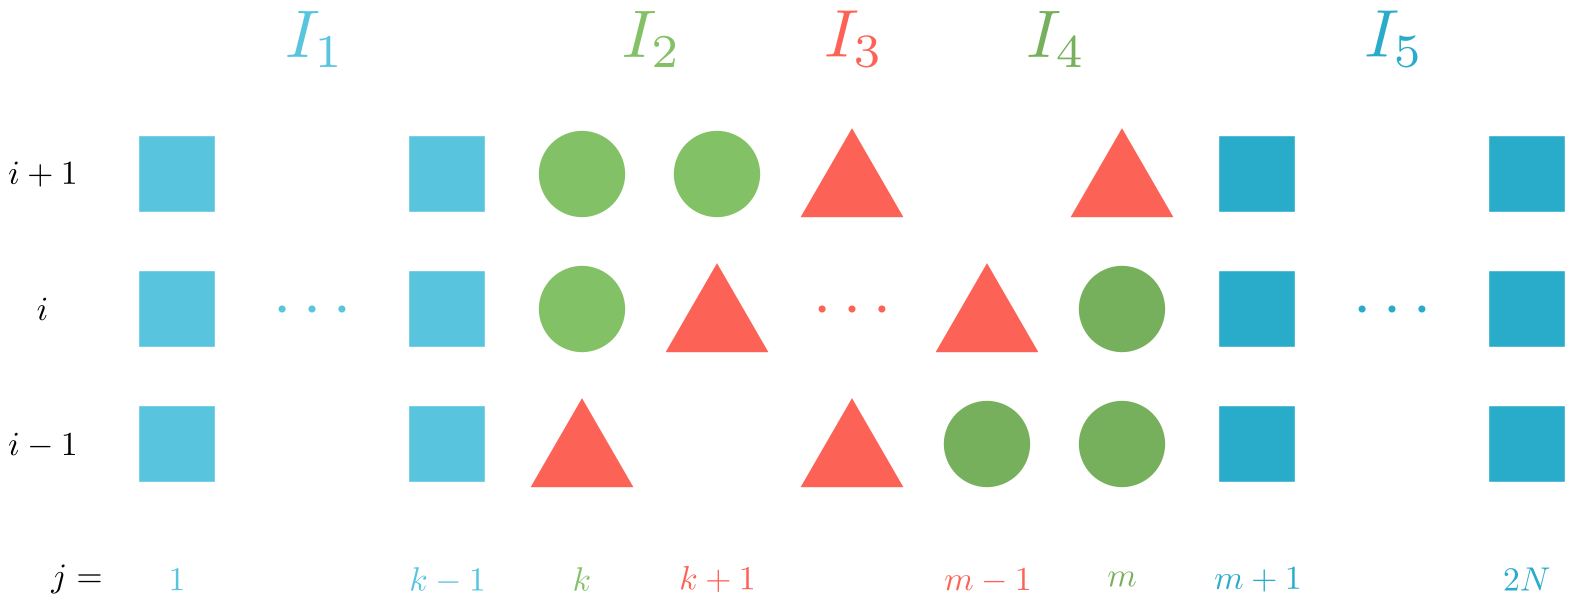
\includegraphics[width=0.7\textwidth]{Depart.png}
  \caption{Natural-Skew ordering of \(R_i\).}
  \label{fig:depart}
\end{figure}

The complexity in estimating \(S_{ij}\) in \eqref{def:Sij} lies in the fact that the integral domains for  \(T_{i-1, j-1}, T_{i,j}\) and \(T_{i+1,j+1}\) are distinct.
We first normalize $T_{ij}$ to the unit interval.

% To estimete \(S_{ij}\), we need some preparations.
\begin{lemma} \label{lmm:Tij-normalized}
  For any \(y\in (x_{j-1}, x_{j})\), there exits % \(y=y_j^\theta\),
  \begin{equation*} %\label{eq:Tij-normal}
    \begin{aligned}
      T_{ij} & = \int_{x_{j-1}}^{x_{j}} (u(y) - \Pi_hu(y)) K(x_i - y) dy  \\
             & = \int_{0}^{1} (u(y_j^\theta) - \Pi_hu(y_j^\theta)) K(x_i - y_j^\theta) h_j d\theta  \\
      %        & = \int_{x_{j-1}}^{x_{j}}
      % -\frac{\theta (1-\theta)}{2} h_j^2 u''(y_j^\theta)\frac{|y_j^\theta-x_i|^{1-\alpha}}{\Gamma(2-\alpha)} \\
      %        & \quad + \frac{\theta (1-\theta)}{3!} h_j^3 \frac{|y_j^\theta-x_i|^{1-\alpha}}{\Gamma(2-\alpha)} ((1-\theta)^2 u'''(\eta_{j1}^\theta) - \theta^2  u'''(\eta_{j2}^\theta)) d y_j^\theta \\
             & = \int_{0}^{1}
      -\frac{\theta (1-\theta)}{2} h_j^3 u''(y_j^\theta) K(x_i - y_j^\theta) d\theta   \\
             & \quad +  \int_{0}^{1} \frac{\theta (1-\theta)}{3!} h_j^4  K(x_i - y_j^\theta) \left( \theta^2 u'''(\eta_{j1}^\theta) - (1-\theta)^2 u'''(\eta_{j2}^\theta) \right) d\theta
    \end{aligned}
  \end{equation*}
  with \(\eta_{j1}^\theta \in (x_{j-1}, y_j^\theta), \eta_{j2}^\theta \in (y_j^\theta, x_j)\).
\end{lemma}
\begin{proof}
  By \eqref{def:Tij} and \Cref{lmm:Dyj}, the desired result is obtained.
\end{proof}

% Given that $j$ varies with $i$ at the indices of $T_{ij}$ within \(S_{ij}\) by \eqref{def:Sij}, we construct functions that satisfy the corresponding property.
To estimate the local truncation error more concisely, we construct the following grid mapping functions.




% \textcolor{purple}{
\begin{definition} 
\label{def:gridmapfunc}
  For \(1\le i, j \le 2N-1\), we define the grid mapping functions
  \begin{equation} \label{def:yij}
    y_{i,j}(x) = \begin{cases}
      (x^{1/r} + Z_{j-i})^r               & i< N, j< N, \\
      \dfrac{x^{1/r} - Z_i}{Z_1} h_N + x_N  & i< N, j=N, \\
      2T - (Z_{2N-(j-i)} - x^{1/r})^r     & i< N, j>N, \\
      \left(\dfrac{Z_1}{h_N}  (x-x_N) + Z_j \right)^r  & i=N, j< N, \\
      x                                   & i=N, j=N, \\
      2T - \left(\dfrac{Z_1}{h_N}  (2T-x-x_N) + Z_{2N-j} \right)^r   & i=N , j > N, \\
      (Z_{2N+j-i} - (2T - x)^{1/r})^r  & i > N, j< N, \\
      \dfrac{Z_{2N-j} - (2T-x)^{1/r}}{Z_1} h_N + x_N  & i > N, j=N, \\
      2T-((2T-x)^{1/r}-Z_{j-i})^r & i > N, j> N \\
    \end{cases}
  \end{equation}
  with  \( Z_{j} := T^{1/r}\frac{j}{N} \).
\end{definition}

Let us further define 
  \begin{equation} \label{def:hij}
    h_{i,j}(x) = y_{i,j}(x) - y_{i,j-1}(x),
  \end{equation}
  \begin{equation} \label{def:yijt}
    y_{i,j}^\theta(x) = (1-\theta) y_{i,j-1}(x) + \theta y_{i,j-1}(x), \quad \theta \in (0, 1),
  \end{equation}
  \begin{equation} \label{def:Pj-itheta-jlN}
    {P_{i,j}^\theta}(x) = ({h_{i,j}}(x))^3  K(x - {y_{i,j}^\theta}(x) ) u''({y_{i,j}^\theta}(x)),
  \end{equation}
  \begin{equation} \label{def:Qj-itheta-jlN}
    {Q_{i,j,l}^{\theta}}(x) = ({h_{i,j}}(x))^l K(x - {y_{i,j}^\theta}(x)), \quad l=3, 4.
  \end{equation}
% }
Then, we can check that
\begin{equation} \label{eq:prop-of-GMFs}
    \begin{gathered}
      y_{i,j}(x_{i-1}) = x_{j-1}, \quad y_{i,j}(x_{i}) = x_{j}, \quad y_{i,j}(x_{i+1}) = x_{j+1}, \\
      h_{i,j}(x_{i-1}) = h_{j-1}, \quad h_{i,j}(x_{i}) = h_j, \quad h_{i,j}(x_{i+1}) = h_{j+1}, \\
      y_{i,j}^\theta(x_{i-1}) = y_{j-1}^\theta, \quad y_{i,j}^\theta(x_{i}) = y_{j}^\theta, \quad y_{i,j}^\theta(x_{i+1}) = y_{j+1}^\theta.
      % y_{i,j} = y_{j,i}^{-1}, \quad y_{k,j} \circ y_{i,k} = y_{i,j},
    \end{gathered}
\end{equation}
% where $f^{-1}$ denotes the inverse function and $f \circ g$ represent the composition of functions which means $f\circ g (x) = f(g(x))$.
Now, we can rewrite \(T_{ij}\) by \eqref{def:Pj-itheta-jlN} in \eqref{lmm:Tij-normalized} as
% \begin{lemma} 
  % For \(0\le i \le 2N\), \(1 \le j \le 2N\),
  \begin{equation} \label{lmm:Tij-express-as-int-of-function}
    \begin{aligned}
      T_{ij} & = \int_{0}^{1} -\frac{\theta (1-\theta)}{2} {P_{i,j}^\theta}(x_i) d\theta    \\
             & \quad + \int_{0}^{1} \frac{\theta (1-\theta)}{3!}{Q_{i,j,4}^\theta}(x_i) \left[ \theta^2  u'''(\eta_{j,1}^\theta) - (1-\theta)^2 u'''(\eta_{j,2}^\theta) \right] d\theta.
    \end{aligned}
  \end{equation}
  From \eqref{def:Dh2}, \eqref{def:Sij} and \eqref{lmm:Tij-express-as-int-of-function}, for \( 1 \le i \le 2N-1\), \(2\le j \le 2N-1\), we have
  \begin{equation} \label{eq:Sij-int}
    \begin{aligned}
      S_{ij}
             & = \int_{0}^{1} -\frac{\theta (1-\theta)}{2} D_h^2 P_{i,j}^\theta(x_i)  d\theta    \\
             & \quad +  \int_{0}^1 \frac{\theta^3 (1-\theta)}{3!} \frac{2}{h_{i} + h_{i+1}}\left( \frac{{Q_{i,j,4}^\theta}(x_{i+1}) u'''(\eta_{j+1,1}^\theta) - {Q_{i,j,4}^\theta}(x_{i}) u'''(\eta_{j,1}^\theta)}{h_{i+1}}\right)  d\theta \\
             & \quad -  \int_{0}^1 \frac{\theta^3 (1-\theta)}{3!} \frac{2}{h_{i} + h_{i+1}}\left( \frac{{Q_{i,j,4}^\theta}(x_{i}) u'''(\eta_{j,1}^\theta) - {Q_{i,j,4}^\theta}(x_{i-1}) u'''(\eta_{j-1,1}^\theta)}{h_{i}}\right)  d\theta   \\
             & \quad -  \int_{0}^1 \frac{\theta (1-\theta)^3}{3!} \frac{2}{h_{i} + h_{i+1}}\left( \frac{{Q_{i,j,4}^\theta}(x_{i+1}) u'''(\eta_{j+1,2}^\theta) - {Q_{i,j,4}^\theta}(x_{i}) u'''(\eta_{j,2}^\theta)}{h_{i+1}}\right)  d\theta \\
             & \quad +  \int_{0}^1 \frac{\theta (1-\theta)^3}{3!} \frac{2}{h_{i} + h_{i+1}}\left( \frac{{Q_{i,j,4}^\theta}(x_{i}) u'''(\eta_{j,2}^\theta) - {Q_{i,j,4}^\theta}(x_{i-1}) u'''(\eta_{j-1,2}^\theta)}{h_{i}}\right)  d\theta.
    \end{aligned}
  \end{equation}
% where the operator $D_h^2$ is defined in .
% \end{lemma}


The derivatives of the grid mapping functions are calculated as follows.
\begin{lemma} \label{lmm:derivatives-of-MTFs}
For $1\le i,j \le 2N-1$, there exist, %by \eqref{def:yij}
  \begin{equation*}
    y_{i,j}'(x) = \begin{cases}
      y_{i,j}^{1-1/r}(x) x^{1/r-1}   ,& i< N, j< N, \\
      \dfrac{h_N}{r Z_1} x^{1/r-1}  ,& i< N, j=N, \\
      (2T-y_{i,j}(x))^{1-1/r} x^{1/r-1}   ,& i< N, j>N, \\
      y_{i,j}^{1-1/r}(x) \dfrac{r Z_1}{h_N}  ,& i=N, j< N, \\
      1   & i=N, j=N ,
    \end{cases}
  \end{equation*}
  and
  \begin{equation*}
    y_{i,j}''(x) = \frac{1-r}{r}
      \begin{cases}
        y_{i,j}^{1-2/r}(x) x^{1/r-2} Z_{j-i}   ,& i< N, j< N, \\
        \dfrac{h_N}{r Z_1} x^{1/r-2}  ,& i< N, j=N, \\
        (2T-y_{i,j}(x))^{1-2/r} x^{1/r-2} Z_{2N-j+i}   ,& i< N, j>N, \\
        -y_{i,j}^{1-2/r}(x) \left(\dfrac{r Z_1}{h_N}\right)^2  ,& i=N, j< N, \\
        0   ,& i=N, j=N .
      \end{cases}
  \end{equation*}
\end{lemma}
\begin{proof}
    The desired results can be obtained by \Cref{def:gridmapfunc} directly.
\end{proof}


% We first give some properties of the grid mapping functions, which will be used.
The following lemmas about the grid mapping functions will be used in next subsection.
They are proved in \Cref{sec:prfs-of-GMFs}.


\begin{lemma} \label{lmm:gen-prop-of-MTFs}
  For any \(\xi \in (x_{i-1}, x_{i+1})\), \(2 \le i,j \le 2N-2\), there exist
  \begin{gather*}
    \xi \simeq x_i, \quad \delta(y_{i,j}(\xi))\simeq \delta(x_j), \quad h_{i,j}(\xi) \simeq h_j, \\
  % \end{equation*}
  % % For \(1\le i, j \le 2N-1\),
  % \begin{equation*}
    |y_{i,j}(\xi) - \xi| \simeq |x_j - x_i|, \quad |y_{i,j-1}(\xi) - \xi| \simeq |x_{j-1} - x_i|, \\
  % \end{equation*}  %then  for \(1\le i\le 2N-1, 2\le j \le 2N-1\),
  % \begin{equation*}
    |y_{i,j}^\theta(\xi) - \xi| = (1-\theta)|y_{i,j-1}(\xi) - \xi| + \theta |y_{i,j}(\xi) - \xi| \simeq |y_j^\theta - x_i|.
  \end{gather*}
\end{lemma}
% \begin{proof}
%     \textcolor{red}{From \Cref{prf:gen-prop-of-MTFs} in Appendix, the desired result } 
% \end{proof}




% \textcolor{red}{
\begin{lemma} \label{lmm:esitmate-of-MTFs-1}
  For any \(\xi \in (x_{i-1}, x_{i+1}) \), \(2\le i \le N, 2\le j \le 2N-2\), there exist
  \begin{equation*}
    |h_{i,j}'(\xi)| \le C (r-1) Z_1 x_i^{1/r-1}  \delta(x_j)^{1-2/r}
    \le C(r-1) h_j x_i^{1/r-1} \delta(x_j)^{-1/r},
  \end{equation*}
  \begin{equation*}
    \left|(y_{i,j}(\xi) - \xi)'\right| \le C x_i^{-1} |x_j - x_i|.
  \end{equation*}
\end{lemma}
% }
% \textcolor{red}{proof from Appendix}


\begin{lemma} \label{lmm:esitmate-of-MTFs-2}
  For any \(\xi \in (x_{i-1}, x_{i+1})\), \(2\le i \le N, 2\le j \le 2N-2\), there exist
  \begin{equation*}
    |y_{i,j}''(\xi)| \le C(r-1)
    \begin{cases}
      x_j^{-1/r} x_i^{1/r-2} |x_j - x_i|  ,& i < N, j < N,  \\
      x_N^{1-1/r} x_i^{1/r-2}             ,& i < N, j = N , \\
      \delta(x_j)^{1-2/r} x_i^{1/r-2} x_N^{1/r}     ,& i < N, j > N , \\
      \delta(x_j)^{1-2/r} x_N^{2/r-2}             ,& i = N, j \neq N , \\
      0   & i = N, j = N.
    \end{cases}
  \end{equation*}
  For \(2\le i \le N, 3\le j \le 2N-2\),  there exist 
  \begin{equation*}
    |h_{i,j}''(\xi)| \le C (r-1)
    \begin{cases}
      Z_1 x_i^{1/r-2} x_j^{-2/r} (|x_j - x_i| + x_j)   ,& i < N, j < N , \\
      x_i^{1/r-2} x_N^{1-1/r}                        ,& i < N, j=N, N+1, \\
      Z_1 x_i^{1/r-2} \delta(x_j)^{1-3/r}  x_N^{1/r}    ,& i < N, j>N+1 ,\\
      Z_1 x_N^{2/r-2} \delta(x_j)^{1-3/r}               ,& i = N, j \neq N, N+1 , \\
      x_N^{-1}                                       ,& i = N, j = N, N+1.
    \end{cases}
  \end{equation*}
\end{lemma}
% \textcolor{red}{proof from Appendix}


% So we first introduce following two lemmas.
% \textcolor{blue}{
  \begin{lemma} \label{lmm:d2Pj-itle}
    % There exists a constant \(C=C(T, \alpha, \beta, r, f)\) such that
    Let \({P_{i,j}^\theta}(x_i)\) be defined by \eqref{def:Pj-itheta-jlN} and the difference quotient operator $D_h^2$ be defined by \eqref{def:Dh2}. Then we have
    \paragraph{Case 1}
    For \(3\le i < N, \lceil\frac{i}{2}\rceil+1 \le j \le \min\{2i-1, N-1\}\), there exists
    \begin{equation*}
      |D_h^2 {P_{i,j}^\theta}(x_{i})| \le C h_j^3 |y_j^\theta - x_i|^{1-\alpha} x_i^{\alpha/2-4}.
    \end{equation*}
    \paragraph{Case 2}
    For \(N/2\le i \le N\), \(j=N, N+1\), there exists
    \begin{equation*}
      \begin{aligned}
        |D_h^2 P_{i,j}^\theta(\xi)| 
        \le C h_j^3 |y_j^\theta - x_i|^{1-\alpha}  + C(r-1) h_j^2 \Big(|y_j^\theta - x_i|^{1-\alpha} + h_j|y_j^\theta - x_i|^{-\alpha}
        \Big).
      \end{aligned}
    \end{equation*}
    \paragraph{Case 3}
    For \(N/2 \le i \le N\), \(N+2 \le j \le 2N-\lceil\frac{N}{2}\rceil\), there exists
    \begin{equation*}
      \begin{aligned}
        |D_h^2 P_{i,j}^\theta(\xi)| 
        \le C h_j^3 \Big(|y_j^\theta - x_i|^{1-\alpha}  + (r-1) |y_j^\theta - x_i|^{-\alpha}
        \Big).
      \end{aligned}
    \end{equation*}
    % \paragraph{Case 4}
    % For \(i=N\), \(N/2 \le j < N\)
    % where \(y_j^\theta = \theta x_{j-1} + (1-\theta) x_{j}\)
  \end{lemma}
% }

  
% \textcolor{blue}{
\begin{lemma} \label{lmm:dQj-itle}
  % There exists a constant \(C=C(T, \alpha, \beta, r, f)\) such that 
  Let \({Q_{i,j, l}^\theta}(x_i)\) be defined by \eqref{def:Qj-itheta-jlN}. Then we have
  for \(2 \le i \le N\), \(2 \le j \le 2N-2\), \(l=3,4\), there exist
  \begin{equation*}
    \begin{aligned}
      & \left| \frac{{Q_{i,j,l}^\theta}(x_{i+1}) u^{(l-1)}(\eta_{j+1}^\theta) - {Q_{i,j,l}^\theta}(x_{i}) u^{(l-1)}(\eta_{j}^\theta)}{h_{i+1}}\right|  \\
      & \quad \le C h_j^l |y_j^\theta - x_i|^{1-\alpha} x_i^{-1} \delta(x_j)^{\alpha/2-l+1-1/r} (x_i^{1/r} + \delta(x_j)^{1/r}),
    \end{aligned}
  \end{equation*}
  and
  \begin{equation*}
    \begin{aligned}
      & \left| \frac{{Q_{i,j,l}^\theta}(x_{i}) u^{(l-1)}(\eta_{j}^\theta) - {Q_{i,j,l}^\theta}(x_{i-1}) u^{(l-1)}(\eta_{j-1}^\theta)}{h_{i}} \right|  \\
      & \quad \le C h_j^l |y_j^\theta - x_i|^{1-\alpha} x_i^{-1} \delta(x_j)^{\alpha/2-l+1-1/r} (x_i^{1/r} + \delta(x_j)^{1/r})
    \end{aligned}
  \end{equation*}
  with \(\eta_{j}^\theta \in (x_{j-1}, x_{j})\).
\end{lemma}
% }









\subsection{Error analysis of $R_i$}
\label{subsec:proofofRi}
In this subsection, we estimate the first term of the local truncation error $R_i$ in \eqref{eq:Ri} through \eqref{eq:departR1R2} and \eqref{eq:depart-Ri}.
We denote
\begin{equation} \label{def:Kyx}
    K_y(x) := K(x-y) = \frac{\kappa_\alpha}{\Gamma(2-\alpha)} |x - y|^{1-\alpha}, \quad 1<\alpha<2,
\end{equation}
where the kernel function $K(x)$ is given in \eqref{def:I2-a} and $\kappa_\alpha$ is given in \eqref{eq:aij}.
% where we choose \(m = 2i\) for \(3 \le i < N/2\), and \(m = N-\lceil N/2 \rceil +1\) for \(N/2 \le i\le N\). 
% in \eqref{eq:depart-Ri}.
% The constants \(C\) of following lemmas in this subsection are all \(C=C(T, \alpha, \beta, r, f)>0\).

% For the second term in \eqref{eq:departR1R2} and \(I_5\) in \eqref{eq:depart-Ri}, we have following results.
\begin{lemma} \label{lmm:Ri-I5-1}
% There exists a constant \(C=C(T, \alpha, \beta, r, f)\) such that
Let \(I_5 = \sum_{j=m+1}^{2N} V_{ij}\) be defined by \eqref{eq:depart-Ri}. Then we have
\paragraph{Case 1}
For  \(1 \le i < N/2\) and \(m=\max\{2i, 3\}\), there exists
\begin{equation*}
  \begin{aligned}
    \sum_{j=m+1}^{2N} \left| V_{ij} \right| 
    \le C h^2 x_i^{-\alpha/2-2/r}
  % \end{aligned}
% \end{equation}
% \paragraph{Case 2}
% For \(1 \le i < N/2\), there exists
% \begin{equation}
  % \begin{aligned}
    % \sum_{j=N+1}^{2N} |V_{ij}|
    + \begin{cases}
          C h^2,             & \alpha/2-2/r+1 > 0, \\
          C h^2 \ln(N) ,     & \alpha/2-2/r+1 = 0, \\
          C h^{r\alpha/2+r}, & \alpha/2-2/r+1 < 0.
        \end{cases}
  \end{aligned}
\end{equation*}
\paragraph{Case 2}
For \(N/2 \le i \le N\) and $m=2N-\lceil \frac{N}{2} \rceil +1$, there exists
\begin{equation*}
  \begin{aligned}
    \sum_{j=m+1}^{2N} |V_{ij}|
    \le \begin{cases}
          C h^2,             & \alpha/2-2/r+1 > 0, \\
          C h^2 \ln(N) ,     & \alpha/2-2/r+1 = 0, \\
          C h^{r\alpha/2+r}, & \alpha/2-2/r+1 < 0.
        \end{cases}
  \end{aligned}
\end{equation*}
\end{lemma}
% \textcolor{red}{correct waiting ...}
\begin{proof}
  % In Case 1, f
  For $1\le i < N/2$, $m+1 \le j \le 2N$ with \(m=\max\{2i, 3\}\),
  using \eqref{def:Tij}, \eqref{def:Vij}, \eqref{def:Kyx}, \Cref{lmm:Dyjleh2ya/2m2/r,lmm:Dh2Kyxi}, we have
  \begin{equation*}
    \begin{aligned}
      | V_{ij}| 
      & =  \left| \int_{x_{j-1}}^{x_{j}}\left( u(y) - \Pi_hu(y)\right) D_h^2 K_y (x_i) dy \right|  \\
      & \le C h^2 \int_{x_{j-1}}^{x_{j}} \delta(y)^{\alpha/2-2/r} |x_i-y|^{-1-\alpha} dy.
            %  & = C h^2 \int_{x_{j-1}}^{x_{j}} y^{-\alpha/2-2/r-1} dy
    \end{aligned}
  \end{equation*}
  Since $y\ge x_{j-1} \ge x_{2i}$, $ y - x_i \simeq y$, and \(x_{i} \simeq x_{2i} \), it yields
  \begin{equation*}
    \begin{aligned}
      \sum_{j=m+1}^{N} |V_{ij}|
        & \le C h^2 \int_{x_{2i}}^{x_{N}} y^{-\alpha/2-2/r-1} dy                     \\
        & = \frac{C}{\alpha/2+2/r} h^2 ( x_{2i}^{-\alpha/2-2/r} - T^{-\alpha/2-2/r}) \\
        & \le C h^2 x_i^{-\alpha/2-2/r}.
    \end{aligned}
  \end{equation*}
  % By \eqref{def:Vij}, \Cref{lmm:Dyjleh2ya/2m2/r}, \Cref{lmm:Dh2Kyxi} and \(y-x_i\simeq T\),
  % \begin{equation*}
  %   \begin{aligned}
  %     |V_{ij}| 
  %     % & = \left| \int_{x_{j-1}}^{x_{j}}(u(y) - \Pi_hu(y)) D_h^2 K_y (x_i) dy \right| \\
  %           %  & \le C \int_{x_{j-1}}^{x_{j}} h^2 (2T-y)^{\alpha/2-2/r} |y-x_i|^{-1-\alpha} dy                                          \\
  %            & \le C h^2  T^{-1-\alpha} \int_{x_{j-1}}^{x_{j}} (2T-y)^{\alpha/2-2/r} dy,
  %   \end{aligned}
  % \end{equation*}
  On the other hand, since $y-x_i \simeq T$ if $y\ge x_N = T$, there exist
  \begin{equation*}
    \begin{aligned}
      \sum_{j=N+1}^{2N-1} |V_{ij}|
       & \le C T^{-1-\alpha} h^2 \int_{x_{N}}^{x_{2N-1}} (2T-y)^{\alpha/2-2/r}  dy                       \\
       % & \le CT^{-1-\alpha} h^2 
       %   \begin{cases}
       %      \frac{1}{\alpha/2-2/r+1} T^{\alpha/2-2/r+1},        
       %      & \alpha/2-2/r+1 > 0 ,\\
       %      \ln(T)-\ln(h_{2N}),   & \alpha/2-2/r+1 = 0 ,\\
       %      \frac{1}{|\alpha/2-2/r+1|} h_{2N}^{\alpha/2-2/r+1}, 
       %      & \alpha/2-2/r+1 < 0,
       %    \end{cases} \\
       & \le \begin{cases}
             \frac{C}{\alpha/2-2/r+1}T^{-\alpha/2-2/r} \; h^2,                & \alpha/2-2/r+1 > 0 ,\\
             CrT^{-1-\alpha} h^2 \ln(N),    & \alpha/2-2/r+1 = 0 ,\\
             \frac{C}{|\alpha/2-2/r+1|} T^{-\alpha/2-2/r} \; h^{r\alpha/2+r}, & \alpha/2-2/r+1 < 0  .
           \end{cases}
    \end{aligned}
  \end{equation*}
  Finally, by \Cref{lmm:Dyj1}, one has
  \begin{equation*}
    |V_{i,2N}| \le C T^{-1-\alpha} h_{2N}^{\alpha/2+1} = C T^{-\alpha/2} h^{r\alpha/2+r}.
  \end{equation*}
  Then, the desired result in Case 1 is obtained.
  We can similarly prove for Case 2, the details are omitted here.
\end{proof}



Immediately, we can calculate $R_1, R_2$ from \eqref{eq:departR1R2}.
\begin{lemma} \label{lmm:R1R2}
For \(i=1, 2\), we have
  \begin{equation*}
    \begin{aligned}
      |R_i| \le C h^2 x_i^{-\alpha/2-2/r} +
      \begin{cases}
        C h^2,             & \alpha/2-2/r+1 > 0 ,\\
        C h^2 \ln(N) ,     & \alpha/2-2/r+1 = 0 ,\\
        C h^{r\alpha/2+r}, & \alpha/2-2/r+1 < 0.
      \end{cases}
    \end{aligned}
  \end{equation*}
\end{lemma}
\begin{proof}
  According to \eqref{eq:departR1R2}, \Cref{lmm:sumSij13,lmm:Ri-I5-1}, the desired result is obtained.
\end{proof}


For \(R_i\) with \(3\le i\le N\), the terms \(\{I_1, I_2, I_3, I_4\}\) in \eqref{eq:depart-Ri} remain to be estimated.
% \textcolor{blue}{
  \begin{lemma} \label{lmm:Ri-I1}
    % There exists a constant \(C=C(T, \alpha, \beta, r, f)\) such that 
    Let \(I_1 = \sum_{j=1}^{k-1} V_{ij}\) be defined by \eqref{eq:depart-Ri}.
    Then we have, 
    for \(3\le i \le N, k=\lceil\frac{i}{2}\rceil\),
    \begin{equation*}
      \sum_{j=1}^{k-1} |V_{ij}| \le \begin{cases}
        C h^2 x_i^{-\alpha/2-2/r} ,        & \alpha/2-2/r+1 > 0, \\
        C h^2 x_i^{-1-\alpha} \ln(i),      & \alpha/2-2/r+1 = 0 ,\\
        C h^{r\alpha/2+r} x_i^{-1-\alpha}, & \alpha/2-2/r+1 < 0.
      \end{cases}
    \end{equation*}
  \end{lemma}
% }
\begin{proof}
  According to \eqref{def:Vij}, \Cref{lmm:Dyj1,lmm:Dh2Kyxi}, it yields
  \begin{equation*}
    |V_{i1}| \le C \int_{0}^{x_1} x_1^{\alpha/2} |x_i-y|^{-1-\alpha}dy \simeq x_1^{\alpha/2+1} x_i^{-1-\alpha} = T^{\alpha/2+1} h^{r\alpha/2+r} x_i^{-1-\alpha}.
  \end{equation*}
  Using \Cref{lmm:Dyjleh2ya/2m2/r}, \Cref{lmm:Dh2Kyxi} and $y\le x_{k-1} < 2^{-r}x_i $, \(x_i - y \simeq x_i\), we have
  \begin{equation*}
    \begin{aligned}
      |V_{ij}| 
      % & = \left|  \int_{x_{j-1}}^{x_{j}}(u(y) - \Pi_hu(y)) D_h^2 K_y(x_i) dy  \right| \\
             \le C h^2 \int_{x_{j-1}}^{x_{j}} y^{\alpha/2-2/r} x_i^{-1-\alpha} dy, \quad 2 \le j \le k-1,
    \end{aligned}
  \end{equation*}
  and
  \begin{equation*}
    \begin{aligned}
      \sum_{j=2}^{k-1} |V_{ij}|
        \le C h^{r\alpha/2+r} x_i^{-1-\alpha} + C h^2 x_i^{-1-\alpha} \int_{x_1}^{x_{\lceil\frac{i}{2}\rceil-1}} y^{\alpha/2-2/r} dy.
    \end{aligned}
  \end{equation*}
  % But \(x_{\lceil\frac{i}{2}\rceil-1} \le 2^{-r} x_i\), s
  Moreover we can check that
  \begin{equation*}
    \begin{aligned}
      \int_{x_1}^{x_{\lceil\frac{i}{2}\rceil-1}} y^{\alpha/2-2/r} dy
       & \le \begin{cases}
               \frac{1}{\alpha/2-2/r+1} (2^{-r} x_i)^{\alpha/2-2/r+1}  ,& \alpha/2-2/r+1 > 0, \\
               \ln(2^{-r} x_i) - \ln(x_1)                              ,& \alpha/2-2/r+1 = 0, \\
               \frac{1}{|\alpha/2-2/r+1|} x_1^{\alpha/2-2/r+1}         ,& \alpha/2-2/r+1 < 0.
             \end{cases}
    \end{aligned}
  \end{equation*}
  The proof is completed.
  % The desired result is proved.
\end{proof}


Subsequently, we turn our attention to $I_3=\sum_{j=k+1}^{m-1} S_{ij}$ 
with $m=2i$ for $3\le i<N/2$ and $m=2N-\lceil N/2 \rceil +1$ for $N/2 \le i \le N$ in \eqref{def:m2c}.
    % \textcolor{blue}{
  \begin{lemma} \label{lmm:estimate-Sij}
  Let \(I_3 = \sum_{j=k+1}^{m-1} S_{ij}\) be defined by \eqref{eq:depart-Ri}. Then we have
    % There exists a constant \(C=C(T, \alpha, \beta, r, f)\)  such that 
    \paragraph{Case 1}
    For \(N/2 \le i \le N\), $m=2N-\lceil N/2 \rceil +1$, there exist
    \begin{equation*}
      |S_{ij}| \le C (h^3 + (r-1)h^2) (T-x_i+h_N)^{1-\alpha}, \quad j=N, N+1,
    \end{equation*}
    % \paragraph{Case 3}
    % For \(N/2 \le i \le N\), %\(N+2 \le j \le 2N-\lceil\frac{N}{2}\rceil\), 
    % there exists
    and
    % \begin{equation*}
    %   |S_{ij}| \le C h^2 \int_{x_{j-1}}^{x_{j}} |y - x_i|^{1-\alpha} + (r-1)|y - x_i|^{-\alpha} dy.
    % \end{equation*}
    % Thus,2N-\lceil\frac{N}{2}\rceil
    \begin{equation*}
      \sum_{j=N+2}^{m-1} \left|S_{ij} \right| 
      \le C h^2 + C (r-1) h^2 (T-x_i + h_N)^{1-\alpha}.
    \end{equation*}
    \paragraph{Case 2}
    For \(3\le i \le N-1\), $k=\lceil \frac{i}{2} \rceil$,  %\(k+1 \le j \le \min\{2i-1, N-1\}\), 
    there exist
    % Thus,
    \begin{equation*}
       \sum_{j=k+1}^{\min\{m-1, N-1\}} \left|S_{ij} \right| \le C h^2 x_i^{-\alpha/2-2/r},
    \end{equation*}
    and
    \begin{equation*}
      \sum_{j=\lceil\frac{N}{2}\rceil+1}^{N-1} \left|S_{Nj} \right| 
      \le C h^2 + C (r-1) h^2 h_N^{1-\alpha}.
    \end{equation*}
    % \paragraph{Case 3} 
  \end{lemma}
  % }
\begin{proof}
% According to \eqref{eq:Sij-int}, %and in each case \(x_i \simeq \delta(x_j)\), \(h_i \simeq h_j\), 
% \Cref{lmm:hilexi,lmm:d2Pj-itle,lmm:dQj-itle}, we have the following:

  Case 1: From \eqref{eq:Sij-int}, using \(\theta(1-\theta) h_j \le |y_j^\theta - x_i|\), \Cref{lmm:hilexi,lmm:d2Pj-itle,lmm:dQj-itle}, it yields
  \begin{equation*}
    \begin{aligned}
      |S_{ij}| &\le C (h_j^3 + (r-1)h_j^2) \int_{0}^1 |y_j^\theta - x_i|^{1-\alpha} d\theta , \quad j=N, N+1
      % &= C (h_j^2 + (r-1)h_j) \int_{x_{j-1}}^{x_{j}} |y - x_i|^{1-\alpha} dy .
    \end{aligned}
  \end{equation*}
  with 
  \begin{equation*}
    \begin{aligned}
      \int_{0}^{1} |y_j^\theta - x_i|^{1-\alpha} dy 
      % &= \frac{1}{2-\alpha} \left((x_j-x_i)^{2-\alpha} - (x_{j-1}-x_i)^{2-\alpha}\right) \\
      &\simeq (|x_j - x_i| + h_N)^{1-\alpha} .
    \end{aligned}
  \end{equation*}

  On the other hand, for $j\ge N+2$, $x_i \simeq x_j \simeq T$, we have
  \begin{equation*}
    \begin{aligned}
      |S_{ij}| &\le C h_j^2 \int_{0}^1 \left(|y_j^\theta - x_i|^{1-\alpha}+ (r-1)|y_j^\theta - x_i|^{-\alpha}\right) h_j d\theta  \\
      &\le C h^2 \int_{x_{j-1}}^{x_{j}} |y - x_i|^{1-\alpha} + (r-1)|y - x_i|^{-\alpha} dy .
    \end{aligned}
  \end{equation*}
  It implies that
  \begin{equation*}
    \begin{aligned}
      \sum_{j=N+2}^{2N-\lceil\frac{N}{2}\rceil} |S_{ij}| 
      &= C h^2 \int_{x_{N+1}}^{x_{2N-\lceil\frac{N}{2}\rceil}} |y - x_i|^{1-\alpha} + (r-1)|y - x_i|^{-\alpha} dy \\
      & \le C h^2 \left( T^{2-\alpha} + (r-1) (T-x_i + h_N)^{1-\alpha} \right)  .
    \end{aligned}
  \end{equation*}
  
Case 2: for $3\le i \le N-1$, $k+1\le j\le \min\{m-1, N-1\}$, using \Cref{lmm:hilexi,lmm:d2Pj-itle,lmm:dQj-itle}, $x_i \simeq x_j$ and $h_i \simeq h_j$, we have
    \begin{equation*} %\label{eq:estimate-Sij-int}
      \begin{aligned}
        |S_{ij}| & \le C h_j^2 x_i^{\alpha/2-4} \int_{0}^{1}  |y_j^\theta - x_i|^{1-\alpha}  h_j d\theta \\
        & =  C h^2 x_i^{\alpha/2-2-2/r} \int_{x_{j-1}}^{x_{j}}  |y - x_i|^{1-\alpha}  dy,
      \end{aligned}
    \end{equation*}
    % Since \(x_k \simeq x_i \simeq x_{\min\{2i-1, N-1\}}\), we have
    and
  \begin{equation*}
    \begin{aligned}
      \sum_{k+1}^{\min\{2i-1, N-1\}} |S_{ij}|
      &\le C h^2 x_i^{\alpha/2-2-2/r} \int_{x_{k}}^{x_{\min\{2i-1, N-1\}}} |y - x_i|^{1-\alpha}  dy    \\
        % & = C h^2 \left( \frac{|x_{k} - x_i|^{2-\alpha}}{\Gamma(3-\alpha)} + \frac{|x_{\min\{2i-1, N-1\}} - x_i|^{2-\alpha}}{\Gamma(3-\alpha)}\right) x_i^{\alpha/2-2-2/r} \\
        & \le C h^2  x_i^{\alpha/2-2-2/r}x_{i}^{2-\alpha} = C h^2 x_i^{-\alpha/2-2/r} .
    \end{aligned}
  \end{equation*}
  We can similarly prove the last inequality by Case 1.
  The proof is completed.
\end{proof}
% Similar to the proof of \Cref{lmm:estimate-Sij}, we have the following remark.
% \begin{remark} \label{rmk:I3i=3}
%     % Especially, for \(i=N\), by symmetry, the estimation of \(\lceil\frac{N}{2}\rceil+1 \le j \le N-1\) is the same as that of \(N+2 \le j \le 2N-\lceil\frac{N}{2}\rceil\).

% \end{remark}

Finally, we focus our error analysis on the terms \(I_2\) and \(I_4\). % in \eqref{eq:depart-Ri} .
\begin{lemma} \label{lmm:Ri-I2-I4-ilN/2}
% There exists a constant \(C=C(T, \alpha, \beta, r, f)\) such that:
% Estimation of \(I_2, I_4\).
Let \(I_2, I_4\) be defined by \eqref{eq:depart-Ri}. Then we have
\paragraph{Case 1}
For \(3\le i \le N\), \(k=\lceil\frac{i}{2}\rceil\), there exists
\begin{equation*}
  I_2 = \frac{2}{h_i + h_{i+1}}
  \left( \frac{1}{h_{i+1}} (T_{i+1, k} +  T_{i+1, k+1})
  - \left(\frac{1}{h_{i}}+\frac{1}{h_{i+1}}\right) T_{i,k} \right) \le C h^2 x_i^{-\alpha/2-2/r} .
\end{equation*}
\paragraph{Case 2}
For \(3\le i < N/2\), $m=2i$, there exists
\begin{equation*}
  I_4 = \frac{2}{h_i + h_{i+1}}
  \left( \frac{1}{h_{i}} (T_{i-1, 2i} +  T_{i-1, 2i-1})
  - \left(\frac{1}{h_{i}}+\frac{1}{h_{i+1}}\right) T_{i,2i} \right) \le C h^2 x_i^{-\alpha/2-2/r} .
\end{equation*}
\paragraph{Case 3}
For \(N/2 \le i \le N\), \(m=N-\lceil\frac{N}{2}\rceil+1\), there exists
\begin{equation*}
  I_4 = \frac{2}{h_i + h_{i+1}}
  \left( \frac{1}{h_{i}} (T_{i-1, m} +  T_{i-1, m-1})
  - \left(\frac{1}{h_{i}}+\frac{1}{h_{i+1}}\right) T_{i,m} \right) \le C h^2 .
\end{equation*}
\end{lemma}
\begin{proof}
Since
\begin{equation} \label{eq:I24-depart}
  \begin{aligned}
     & \frac{1}{h_{i+1}} \left(T_{i+1, k} +  T_{i+1, k+1}\right)
    - \left(\frac{1}{h_{i}}+\frac{1}{h_{i+1}}\right) T_{i,k}   \\
     & = \frac{1}{h_{i+1}} \left(T_{i+1, k} -  T_{i, k}\right) + \frac{1}{h_{i+1}} \left(T_{i+1, k+1} -  T_{i, k}\right) + \left(\frac{1}{h_{i+1}} - \frac{1}{h_{i}}\right) T_{i,k} .
  \end{aligned}
\end{equation}
According to \(x_i - x_k \simeq x_i \simeq x_k\), \Cref{lmm:Dyjleh2ya/2m2/r,lmm:Dh2Kyxi,lmm:hilexi}, we have
\begin{equation*}
  \begin{aligned}
    \frac{1}{h_{i+1}} (T_{i+1, k} -  T_{i, k})
     & = \int_{x_{k-1}}^{x_k} (u(y)-\Pi_hu(y)) D_h K_y (x_i) dy \\
    %  & \le h_k^2 \textcolor{red}{\max_{\eta\in (x_{k-1}, x_k)}|u''(\eta)|} \int_{x_{k-1}}^{x_k} \frac{|\xi-y|^{-\alpha}}{\Gamma(1-\alpha)} dy, \quad \xi\in(x_i, x_{i+1})    \\
     & \le C  h_k^2 x_{k}^{\alpha/2-2} \; h_k|x_i-x_{k}|^{-\alpha}
     \le C  h^2 x_i^{-\alpha/2-2/r} h_k .
  \end{aligned}
\end{equation*}
% which implies that
% \begin{equation*}
  % \frac{2}{h_i + h_{i+1}} \frac{1}{h_{i+1}} |T_{i+1, k} -  T_{i, k}| \le C h^2 x_i^{-\alpha/2-2/r} .
% \end{equation*}

From \Cref{lmm:Dyj,lmm:Tij-normalized} and \eqref{def:Qj-itheta-jlN}, %similar with \eqref{lmm:Tij-express-as-int-of-function}, 
we can obtain
\begin{equation*}
  \begin{aligned}
    \frac{1}{h_{i+1}} \left(T_{i+1, k+1} -  T_{i, k}\right) % \frac{T_{i+1, k+1} -  T_{i, k}}{h_{i+1}}
     & = \int_{0}^{1} \frac{\theta(\theta-1)}{2} \frac{Q_{i,k;3}^\theta(x_{i+1})u''(\eta_{k+1}^\theta) - Q_{i,k;3}^\theta(x_i) u''(\eta_{k}^\theta)}{h_{i+1}} d\theta 
  \end{aligned}
\end{equation*}
with \(\eta_{k}^\theta \in (x_{k-1}, x_k)\) and \(\eta_{k+1}^\theta \in (x_k, x_{k+1})\).
Using \Cref{lmm:dQj-itle,lmm:hilexi}, we have
\begin{equation*}
  % \frac{2}{h_i + h_{i+1}}  
  \frac{1}{h_{i+1}} |T_{i+1, k+1} -  T_{i, k}| \le C h^2 x_i^{-\alpha/2-2/r} h_k.
\end{equation*}

For the third term in \eqref{eq:I24-depart}, using $h_i \simeq h_k$, \Cref{lmm:hilexi,lmm:hi1-hi,lmm:Dyjleh2ya/2m2/r}, it yields
\begin{equation*}
  \begin{aligned}
    % \frac{2}{h_i + h_{i+1}} 
    \frac{h_{i+1}-h_{i}}{h_i h_{i+1}} T_{i,k}
     & \le C(r-1) h_i^{-2} h^2 x_i^{1-2/r} \; h_k^3 x_{k}^{\alpha/2-2} |x_{k}-x_i|^{1-\alpha} \\
     & \le C(r-1) h^2 x_i^{-\alpha/2-2/r} h_k.
  \end{aligned}
\end{equation*}
% Summarize, we have
% \(
%   I_2 \le C h^2 x_i^{-\alpha/2-2/r}.
% \)
Then, the desired result of Case 1 is obtained.
The Case 2 and Case 3 for \(I_4\) can be similarly proven as the way in Case 1; the details are omitted here.
\end{proof}



% Now we have studied every part for proving \Cref{thm:Ri-ilessN/2,thm:Ri-N/2le-i-leN}.

\begin{proof} [\bf Proof of \Cref{thm:Ri-ilessN/2}]
For \(1\le i < N/2\) 
with $m=2i$ in \eqref{eq:depart-Ri}, 
combining
\Cref{lmm:R1R2}, 
\Cref{lmm:Ri-I1}, 
Cases 1 and 2 of \Cref{lmm:Ri-I2-I4-ilN/2}, 
Case 2 of \Cref{lmm:estimate-Sij} and
Case 1 of \Cref{lmm:Ri-I5-1}, 
the proof is completed.
\end{proof}

\begin{proof} [\bf Proof of \Cref{thm:Ri-N/2le-i-leN}]
For \(N/2 \le i \le N \) 
with $m=2N-\lceil N/2 \rceil +1$ in \eqref{eq:depart-Ri},
we split \(I_3\) as
 \begin{equation} \label{eq:I3-depart}
  \begin{aligned}
    I_3 &= \sum_{j=k+1}^{m-1} S_{ij}
         = \sum_{j=k+1}^{N-1} S_{ij} + (S_{iN}+S_{i,N+1}) + \sum_{j=N+2}^{m-1}  S_{ij}.
  \end{aligned}
\end{equation}
According to
\Cref{lmm:Ri-I1}, 
Cases 1 and 3 of \Cref{lmm:Ri-I2-I4-ilN/2}, 
\Cref{lmm:estimate-Sij}
and 
Case 2 of \Cref{lmm:Ri-I5-1}, 
the desired result is obtained.
\end{proof}




% \newpage
\section{Convergence analysis}
\label{sec:proof-convergence}

% We prove the convergency and estimate the global error of our difference-quadrature scheme in this section.
% In this section, we demonstrate the convergence of our difference-quadrature scheme and provide an estimate of its global error.
We can now prove our main convergence result for \Cref{thm:convergence}.

\subsection{Some properties of the stiffness matrix}

% Review the numerical scheme \eqref{def:discrete_equation} and . 
In this subsection, we show some properties of the stiffness matrix \(A\) defined by \eqref{eq:equation_matrix} and construct an appropriate  right-preconditioner for the resulting matrix algebraic equation.


% \begin{definition}
  % We first define an \(M\) matrix as a matrix \textcolor{red}{cite} whose entries are positive on the main diagonal and non-positive elsewhere, and which is strictly row diagonally dominant.
% \end{definition}
% Then we have
\begin{lemma} \label{lmm:AisM}
  The stiffness matrix \(A\) defined by \eqref{eq:equation_matrix} is strictly diagonally dominant, with positive entries on the main diagonal and negative off-diagonal entries.
  In particular, there exists a constant \(C_A\) such that
  \begin{equation*}
    \begin{aligned}
      % S_i := &
      \sum_{j=1}^{2N-1} a_{ij}
      % =      & -\kappa_\alpha \sum_{j=1}^{2N-1}  \frac{2}{h_i + h_{i+1}} \left( \frac{1}{h_{i+1}} \tilde{a}_{i+1,j} - (\frac{1}{h_{i}}+\frac{1}{h_{i+1}})\tilde{a}_{i,j} + \frac{1}{h_{i}} \tilde{a}_{i-1,j}\right) \\
      \ge  C_A (x_i^{-\alpha} + (2T-x_i)^{-\alpha}) 
    \end{aligned}
  \end{equation*}
  with
  % \begin{equation*}
      % C_A = \min \left\{ \frac{2\kappa_\alpha}{\Gamma(4-\alpha)} \frac{1+(2^r-1)^{3-\alpha} + 2(2^r-1) - (2^r)^{3-\alpha} }{2^r (2^r-1)}, \frac{\kappa_\alpha(\alpha-1)}{\Gamma(2-\alpha)} 2^{-r\alpha} \right\} .
  % \end{equation*}
  $C_A = \frac{\kappa_\alpha(\alpha-1)}{\Gamma(2-\alpha)} 2^{-r\alpha}$ .
\end{lemma}
\begin{proof}
Let $C_j := \left( \frac{1}{h_j}, -\frac{1}{h_j}-\frac{1}{h_{j+1}}, \frac{1}{h_{j+1}} \right)$
and
\begin{equation*}
    D_{ij} := \begin{pmatrix}
        |x_{i-1} - x_{j-1}|^{3-\alpha} & |x_{i-1} - x_{j}|^{3-\alpha} &|x_{i-1} - x_{j+1}|^{3-\alpha} \\
        |x_{i} - x_{j-1}|^{3-\alpha} & |x_{i} - x_{j}|^{3-\alpha} &|x_{i} - x_{j+1}|^{3-\alpha} \\
        |x_{i+1} - x_{j-1}|^{3-\alpha} & |x_{i+1} - x_{j}|^{3-\alpha} &|x_{i+1} - x_{j+1}|^{3-\alpha}
    \end{pmatrix} .
\end{equation*}
From \eqref{eq:aij}, we have 
\begin{equation*}
    a_{ij} = \frac{-\kappa_\alpha}{\Gamma(4-\alpha)}\frac{2}{h_i+h_{i+1}} C_i D_{ij} C_j^T  
\end{equation*}
% Then we have
% Let's consider the sign of the elements of $a_{ij}$. 
with $\text{sign}(a_{ij}) = \text{sign}(a_{ji})$.
For \(i=j\), there exists
 \begin{equation*}
     a_{ii} = \frac{\kappa_\alpha}{\Gamma(4-\alpha)}\frac{4}{h_i h_{i+1}} \left( h_i^{2-\alpha} + h_{i+1}^{2-\alpha} - (h_i+h_{i+1})^{2-\alpha} \right) > 0,
 \end{equation*}
 where we use $ 1 + t^\theta >  (1+t)^\theta$ with $t=\frac{h_{i+1}}{h_{i}}$ for $\theta\in (0,1)$.
 
 For \(j = i-1\), we can check that
 % \begin{equation*}
 %     D_{i,i-1} = \begin{pmatrix}
 %        h_{i-1}^{3-\alpha} & 0 &  h_i^{3-\alpha} \\
 %        (h_{i-1} + h_{i})^{3-\alpha} & h_{i}^{3-\alpha} & 0 \\
 %        (h_{i-1} + h_{i}  + h_{i-1})^{3-\alpha} & (h_{i} + h_{i+1})^{3-\alpha} & h_{i+1}^{3-\alpha}
 %    \end{pmatrix} ,
 % \end{equation*}
 % which implies that
 \begin{equation*}
     \begin{aligned}
         C_i D_{i,i-1} C_{i-1}^T
         &= \frac{1}{h_{i-1} h_{i} h_{i+1}} \Big(
            h_{i+1} h_{i-1}^{3-\alpha} - (h_{i}+h_{i+1})(h_{i-1}+h_{i})^{3-\alpha}     \\
            & + h_i(h_{i-1} + h_{i}  + h_{i-1})^{3-\alpha} + (h_{i-1}+h_{i}) (h_{i}+h_{i+1})h_i^{2-\alpha}  \\
            &- (h_{i-1}+h_{i})(h_{i} + h_{i+1})^{3-\alpha}  + h_{i-1} h_{i+1} h_{i}^{2-\alpha} + h_{i-1} h_{i+1}^{3-\alpha}
         \Big) .
     \end{aligned}
 \end{equation*}
 Let \(s = \frac{h_{i-1}}{h_{i}}\) and \(t=\frac{h_{i+1}}{h_{i}}\). 
 Then by \Cref{eq:ineq_fxy}, we have
 \begin{equation*}
     \begin{aligned}
         C_i D_{i,i-1} C_{i-1}^T &= \frac{ h_{i}^{3-\alpha }}{h_{i-1} h_{i+1}} 
         \Big( st(1+s^{2-\alpha} +t^{2-\alpha}) + (1+s+t)^{3-\alpha}    \\
         &- (1+s)(1+t)\left( (1+s)^{2-\alpha} + (1+t)^{2-\alpha} - 1 \right)  \Big) > 0  ,
     \end{aligned}
 \end{equation*}
 which implies that 
 \[a_{i, i-1} = \frac{-\kappa_\alpha}{\Gamma(4-\alpha)}\frac{2}{h_i+h_{i+1}} C_i D_{i,i-1} C_{i-1}^T < 0 .\]
 
 For $|i-j|\ge 2$, $x_{i+1} - y$, $x_{i} - y$ and $x_{i-1} - y$ have the same sign ($> 0$ or $< 0$) for $y\in (x_{j-1}, x_{j+1})$, it yields
 \begin{equation*}
     \frac{h_i}{h_{i}+h_{i+1}} |x_{i+1} - y| +  \frac{h_{i+1}}{h_{i}+h_{i+1}} |x_{i-1} - y| = |x_i - y|.
 \end{equation*}
 Since $x^{1-\alpha}$ is a convex function for $\alpha\in(1,2)$, by Jensen's inequality, we have
 \begin{equation*}
     \frac{h_i}{h_{i}+h_{i+1}} |x_{i+1} - y|^{1-\alpha} +  \frac{h_{i+1}}{h_{i}+h_{i+1}} |x_{i-1} - y|^{1-\alpha} > |x_i - y|^{1-\alpha},
 \end{equation*}
  % \(K_y(x)\) is convex for \(x\in [x_{i-1}, x_{i+1}]\), so 
 which implies that \(D_h^2 K_y(x_i) > 0\) 
 by \eqref{def:Dh2} and \eqref{def:Kyx}.
 Thus, from \eqref{eq:aij}, we get
 \begin{equation*}
     a_{ij} = - D_h^2 I^{2-\alpha} \phi_j (x_i)
      = - \int_{x_{j-1}}^{x_{j+1}} \phi_j(y) D_h^2 K_y(x_i) dy < 0 .
 \end{equation*}


 % Before studying $\sum_{j=1}^{2N-1} a_{ij}$, let's consider $\sum_{j=1}^{2N-1} \tilde{a}_{ij}$ first.
 We next prove that the stiffness matrix \(A\) defined by \eqref{eq:equation_matrix} is strictly diagonally dominant.
 For the quadrature coefficients $\tilde{a}_{ij}$ in \eqref{eq:aij}, we calculate that
  \begin{equation*}
    \begin{aligned}
      \sum_{j=1}^{2N-1} \tilde{a}_{ij}
      = g_0(x_i) + g_{2N}(x_i) 
        % & =  \frac{\kappa_\alpha}{\Gamma(4-\alpha)} \left( \frac{|x_i-x_0|^{3-\alpha} - |x_i-x_1|^{3-\alpha}}{h_1} + \frac{|x_{2N}-x_i|^{3-\alpha} - |x_{2N-1}-x_i|^{3-\alpha}}{h_{2N}} \right) .
    \end{aligned}
  \end{equation*}
  with
  % \begin{equation*}
  %   g(x) = g_{0}(x) + g_{2N}(x) ,
  % \end{equation*}
  % where
  \begin{gather*}
    g_{0}(x) = \frac{-\kappa_\alpha}{\Gamma(4-\alpha)} \frac{|x-x_0|^{3-\alpha} - |x-x_1|^{3-\alpha}}{h_1} ,   \\
    g_{2N}(x) = \frac{-\kappa_\alpha}{\Gamma(4-\alpha)} \frac{|x_{2N}-x|^{3-\alpha} - |x_{2N-1}-x|^{3-\alpha}}{h_{2N}}.
  \end{gather*}
  % Thus
  % \(
  %   -\kappa_\alpha \sum_{j=1}^{2N-1} \tilde{a}_{ij} =  .
  % \)
  % So, by \eqref{eq:aij}
  % Then, for \(2\le i\le 2N-2\),
  It implies that
  \begin{equation*}
    \begin{aligned}
      % S_i = & 
      \sum_{j=1}^{2N-1}a_{ij}        
      % =      & \frac{2}{h_i + h_{i+1}} \left( \frac{1}{h_{i+1}} g(x_{i+1}) - (\frac{1}{h_{i}}+\frac{1}{h_{i+1}})g(x_{i}) + \frac{1}{h_{i}} g(x_{i-1}) \right) \\
      =     D_h^2 g_0(x_i) + D_h^2 g_{2N}(x_i) .
    \end{aligned}
  \end{equation*}
  
  For \(i=1\), there exists
  \begin{equation*}
    \begin{aligned}
      D_h^2 g_0(x_1) &= \frac{2}{h_{1} + h_{2}} \left( \frac{1}{h_{2}} g_0(x_{2}) - (\frac{1}{h_{1}}+\frac{1}{h_{2}})g_0(x_{1}) + \frac{1}{h_{1}} g_0(x_{0}) \right)                                                       \\
      % =                       & \frac{2\kappa_\alpha}{\Gamma(4-\alpha)} \frac{h_1^{3-\alpha}+h_2^{3-\alpha} + 2h_1^{2-\alpha}h_2 - (h_1+h_2)^{3-\alpha} }{(h_{1} + h_{2})h_1 h_2}                          \\
      % =                       & \frac{2\kappa_\alpha}{\Gamma(4-\alpha)} \frac{h_1^{3-\alpha}+h_2^{3-\alpha} + 2h_1^{2-\alpha}h_2 - (h_1+h_2)^{3-\alpha} }{(h_{1} + h_{2})h_1^{1-\alpha} h_2} h_1^{-\alpha} \\
        &= \frac{2\kappa_\alpha}{\Gamma(4-\alpha)} \frac{1+(2^r-1)^{3-\alpha} + 2(2^r-1) - (2^r)^{3-\alpha} }{2^r (2^r-1)} x_1^{-\alpha} \\
        &\ge  \frac{\kappa_\alpha(\alpha-1)}{\Gamma(2-\alpha)}2^{-r\alpha} x_1^{-\alpha} ,
    \end{aligned}
  \end{equation*}
  % where the last inequality can be get from the fact that
  since
  $ h(t) = 2\left( 1+(t-1)^{3-\alpha} + 2(t-1) - t^{3-\alpha} \right) - (3-\alpha)(2-\alpha)(\alpha-1)( t^{2-\alpha} - t^{1-\alpha}) $ is a increasing function for $t=2^r\ge 1$ and $h(1)=0$.
  % with
  % \(
    % 2\left(1+(2^r-1)^{3-\alpha} + 2(2^r-1) - (2^r)^{3-\alpha}\right) > (3-\alpha)(2-\alpha)(\alpha-1)2^{r(1-\alpha}(2^r-1)
  % \) for $r\ge 1$. % we get \(D_h^2 g_0(x_1) > C_A x_1^{-\alpha}\).

  For \(i \ge 2\), using \Cref{lmm:Dh2simd2}, it leads to
  \begin{equation*}
    \begin{aligned}
      D_h^2 g_0(x_i) &=  g_0''(\xi) , \quad \xi \in (x_{i-1}, x_{i+1}) \\
                 & =  -\kappa_\alpha \frac{|\xi-x_0|^{1-\alpha} - |\xi-x_1|^{1-\alpha}}{\Gamma(2-\alpha)h_1}                                               \\
                 & = \frac{\kappa_\alpha(\alpha-1)}{\Gamma(2-\alpha)}  |\xi-\eta|^{-\alpha} , \quad \eta\in [x_0, x_1]                                              \\
                 & \ge \frac{\kappa_\alpha(\alpha-1)}{\Gamma(2-\alpha)} x_{i+1}^{-\alpha}  
                 \ge \frac{\kappa_\alpha(\alpha-1)}{\Gamma(2-\alpha)} 2^{-r\alpha} x_{i}^{-\alpha} .
    \end{aligned}
  \end{equation*}
  Then we have
  \(
    D_h^2 g_0(x_i) \ge C_A x_i^{-\alpha}
  \) with $C_A = \frac{\kappa_\alpha (\alpha-1)}{\Gamma(2-\alpha)}2^{-r\alpha} $ for $i\ge 1$.
  We can similarly prove
  \(
    D_h^2 g_{2N}(x_i) \ge C_A (2T-x_i)^{-\alpha} 
  \). The proof is completed.
\end{proof}



Let us first introduce the quasi-preconditioner
% \begin{equation} \label{def:hat}
%   \delta(x) = \begin{cases}
%     x, & 0<x\le T \\ 2T-x , & T<x<2T
%   \end{cases}
% \end{equation}
% And define
\begin{equation} \label{def:G}
  G = \text{diag}(\delta(x_1), ..., \delta(x_{2N-1})),
\end{equation}
where $\delta(x)$ is defined by \eqref{def:delta}.
Then we have
\begin{lemma} \label{lmm:AGhasSingularity}
  Let \(\tilde{B}:= AG\) and $A$ be defined by \eqref{eq:equation_matrix}. 
  Then the matrix $\tilde{B} = (\tilde{b}_{ij}) \in \mathbb{R}^{(2N-1) \times (2N-1)}$ has positive entries on the main diagonal and negative off-diagonal entries.
  In particular, there exist constants \(C_{\tilde{B}}, C_B\) such that
  \begin{equation*}
    % M_i := 
    \sum_{j=1}^{2N-1} \tilde{b}_{ij}
    \ge  C_B (T - \delta(x_{i}) + h_N)^{1-\alpha} -C_{\tilde{B}} (x_i^{1-\alpha} + (2T-x_i)^{1-\alpha}) .
  \end{equation*}
  with
  % \begin{gather*} 
  \(
    C_B = \frac{2\kappa_\alpha}{\Gamma(2-\alpha)}, \;
    % C_{\tilde{B}} = \max \left\{\frac{2\kappa_\alpha}{\Gamma(4-\alpha)}\frac{2^{r(2-\alpha)} -1}{2^r-1}, \frac{\kappa_\alpha}{\Gamma(2-\alpha)} 2^{r(\alpha-1)} \right\}. 
    C_{\tilde{B}} = \frac{\kappa_\alpha}{\Gamma(2-\alpha)} 2^{r(\alpha-1)} \). 
  % \end{gather*}
\end{lemma}
\begin{proof}
  From \eqref{eq:aij} and \eqref{def:G}, it yields
  \begin{equation*}
    \tilde{b}_{ij} = a_{ij} \delta(x_j) = -  \frac{2}{h_i + h_{i+1}} \left( \frac{1}{h_{i+1}} \tilde{a}_{i+1,j} - (\frac{1}{h_{i}}+\frac{1}{h_{i+1}})\tilde{a}_{i,j} + \frac{1}{h_{i}} \tilde{a}_{i-1,j}\right) \delta(x_j).
  \end{equation*}
  Since
  \(
    \delta(x) \equiv \Pi_h \delta(x) = \sum_{j=1}^{2N-1} \phi_j(x) \delta(x_j)
  \) by \eqref{def:interp} and \eqref{def:delta},
  from the definition of the quadrature coefficients $\tilde{a}_{ij}$ in \eqref{eq:aij}, we have
  \begin{equation*}
    \begin{aligned}
      \sum_{j=1}^{2N-1} \tilde{a}_{ij} \delta(x_j)
                  & = \sum_{j=1}^{2N-1} I^{2-\alpha} \phi_j(x_i) \delta(x_j) 
                    % = I^{2-\alpha} \Pi_h \delta(x_i)
                    = I^{2-\alpha} \delta(x_i)
                  =  -p(x_i) + q(x_i)
                  % & = \frac{-2 \kappa_\alpha}{\Gamma(4-\alpha)}|T-x_i|^{3-\alpha} + \frac{\kappa_\alpha}{\Gamma(4-\alpha)}(x_i^{3-\alpha} + (2T-x_i)^{3-\alpha}) \\
    \end{aligned}
  \end{equation*}
  with
  \begin{equation*}
      p(x) = \frac{2 \kappa_\alpha}{\Gamma(4-\alpha)}|T-x|^{3-\alpha} \quad \text{and} \quad
      q(x) = \frac{\kappa_\alpha}{\Gamma(4-\alpha)}\left( x^{3-\alpha} + (2T-x)^{3-\alpha} \right).
  \end{equation*}

  Thus, we have
  \begin{equation*}
    \begin{aligned}
      % M_i & := 
      \sum_{j=1}^{2N-1} \tilde{b}_{ij} =\sum_{j=1}^{2N-1} a_{ij} \delta(x_j)     
        % &= -\kappa_\alpha\frac{2}{h_i + h_{i+1}}\left(\frac{1}{h_{i+1}} \tilde{M}_{i+1} - (\frac{1}{h_{i}}+\frac{1}{h_{i+1}})\tilde{M}_{i} + \frac{1}{h_{i}} \tilde{M}_{i-1}\right)  \\
      %     & = -\kappa_\alpha\frac{2}{h_i + h_{i+1}}
      % \left( \frac{1}{h_{i+1}} w(x_{i+1})
      % - (\frac{1}{h_{i}}+\frac{1}{h_{i+1}}) w(x_{i})
      % +  \frac{1}{h_{i}} w(x_{i-1}) \right)
       =  D_h^2  p (x_i) -  D_h^2 q(x_i) .
    \end{aligned}
  \end{equation*}
  For \(i \neq N\), by \Cref{lmm:Dh2simd2}, it leads to
  \begin{equation*}
    \begin{aligned}
      D_h^2 p(x_i) 
      % & := -\kappa_\alpha\frac{2}{h_i + h_{i+1}}
      % \left( \frac{1}{h_{i+1}} p(x_{i+1})
      % - (\frac{1}{h_{i}}+\frac{1}{h_{i+1}}) p(x_{i})
      % +  \frac{1}{h_{i}} p(x_{i-1}) \right)     \\
            & = \frac{2 \kappa_\alpha}{\Gamma(2-\alpha)} |T - \xi|^{1-\alpha}  \quad \xi \in (x_{i-1}, x_{i+1}) \\
            & \ge C_B (T - \delta(x_{i}) + h_N)^{1-\alpha} \;\; \text{with} \;\; C_B=\frac{2 \kappa_\alpha}{\Gamma(2-\alpha)},
    \end{aligned}
  \end{equation*}
  % and
  % \begin{equation}
  %   \begin{aligned}
  %     D_h^2 (-\kappa_\alpha p)(x_{N-1}) & := \frac{-2\kappa_\alpha}{h_{N-1} + h_{N}}
  %     \left( \frac{1}{h_{N}} p(x_{N})
  %     - (\frac{1}{h_{N-1}}+\frac{1}{h_{N}}) p(x_{N-1})
  %     +  \frac{1}{h_{N-1}} p(x_{N-2}) \right)                                                                                                                                   \\
  %             & = \frac{2 \kappa_\alpha}{\Gamma(4-\alpha)} \frac{2}{h_{N-1} + h_{N}}
  %     \left( - (\frac{1}{h_{N-1}}+\frac{1}{h_{N}}) h_N^{3-\alpha}
  %     +  \frac{1}{h_{N-1}} (h_{N-1}+h_{N})^{3-\alpha} \right)                                                                                                                   \\
  %             & = \frac{4 \kappa_\alpha}{\Gamma(4-\alpha) h_{N-1}}
  %     \left( - h_{N}^{2-\alpha}
  %     +  (h_{N-1}+h_{N})^{2-\alpha} \right)                                                                                                                                     \\
  %             & = \frac{4 \kappa_\alpha}{(3-\alpha)\Gamma(2-\alpha)} \xi^{1-\alpha}    \quad \xi \in [h_N, h_{N-1}+h_{N}]                                                       \\
  %             & \ge \frac{4 \kappa_\alpha}{(3-\alpha)\Gamma(2-\alpha)} (h_{N-1}+h_{N})^{1-\alpha} = \frac{4 \kappa_\alpha}{(3-\alpha)\Gamma(2-\alpha)} (T - x_{N-2})^{1-\alpha}
  %   \end{aligned}
  % \end{equation}
  and for $i=N$, it yields
  \begin{equation*}
    \begin{aligned}
      D_h^2 p(x_N) 
      % & := -\kappa_\alpha \frac{2}{h_N + h_{N+1}}
      % \left( \frac{1}{h_{N+1}} p(x_{N+1})
      % - (\frac{1}{h_{N}}+\frac{1}{h_{N+1}}) p(x_{N})
      % +  \frac{1}{h_{N}} p(x_{N-1}) \right)                                   \\
          & = \frac{4 \kappa_\alpha}{\Gamma(4-\alpha) h_N^2} h_N^{3-\alpha}
          % = \frac{4 \kappa_\alpha}{\Gamma(4-\alpha)} (T - \delta(x_N)+h_N)^{1-\alpha} .
          \ge C_B (T - \delta(x_N)+h_N)^{1-\alpha} .
    \end{aligned}
  \end{equation*}

  % Symmetrically for \(i\ge N\), we get
  % \begin{equation} \label{eq:|T-xi-1|1-a}
  %   D_h^2(-\kappa_\alpha p)(x_i)\ge \frac{2\kappa_\alpha}{\Gamma(2-\alpha)} (T - \delta(x_{i}) + h_N)^{1-\alpha} .
  % \end{equation}

  We can similarly prove the following inequality.
  \begin{equation*}
    \begin{aligned}
      D_h^2 q(x_i) 
      % & := \frac{2}{h_i + h_{i+1}}
      % \left( \frac{1}{h_{i+1}} q(x_{i+1})
      % - (\frac{1}{h_{i}}+\frac{1}{h_{i+1}}) q(x_{i})
      % +  \frac{1}{h_{i}} q(x_{i-1}) \right) \\
          & \le C_{\tilde{B}}  (x_{i}^{1-\alpha} + (2T-x_{i})^{1-\alpha}), \quad i=1,\cdots, 2N-1 
    \end{aligned}
  \end{equation*}
  % \textcolor{red}{
  The proof is completed.
\end{proof}


Noted that $\tilde{B}=AG$ in \Cref{lmm:AGhasSingularity} is not diagonally dominant, e.g., 
$\sum_{j=1}^{2N-1} \tilde{b}_{ij} < 0 $ if $x_i$ is near the boundary.
We introduce the preconditioner $\lambda I + \mu G$ as following.
% Notice that
% \(
%   x_i^{-\alpha} \ge (2T)^{-1} x_i^{1-\alpha}
% \),
% We have
\begin{lemma}\label{thm:ALGisM}
  % Then the matrix 
  % There exists a constant \(\lambda=\lambda(\alpha, r)\) such that 
  Let \(B := A(\lambda I+\mu G)\) 
    with $\lambda= 1+ 2^{r(\alpha-1)} T $, $\mu = (\alpha-1)2^{-r\alpha-1}$. 
% with \(\lambda = (C_B + 2T C_{\tilde{B}})/C_{A} \). 
  Then the matrix $B = (b_{ij})\in \mathbb{R}^{(2N-1) \times (2N-1)}$ is strictly diagonally dominant, with positive entries on the main diagonal and negative off-diagonal entries.
  In particular, there exists
  \begin{equation*}
    % M_i := 
    \sum_{j=1}^{2N-1} b_{ij} \ge C_A \left( (x_i^{-\alpha} + (2T-x_i)^{-\alpha}) + (T - \delta(x_{i}) + h_N)^{1-\alpha} \right).
  \end{equation*}
\end{lemma}
\begin{proof}
  % calculate $\lambda= 1+ 2^{r(\alpha-1)} T $, $\mu = (\alpha-1)2^{-r\alpha-1}$.
  From \Cref{lmm:AisM,lmm:AGhasSingularity}, we have 
  \begin{equation*}
      \begin{aligned}
          \sum_{j=1}^{2N-1} b_{ij} &= \sum_{j=1}^{2N-1} \left(\lambda a_{ij} + \mu \tilde{b}_{ij} \right) \\
           & \ge \lambda C_A \left( x_i^{-\alpha} + (2T-x_i)^{-\alpha} \right)
            - \mu C_{\tilde{B}} 2T \left( x_i^{-\alpha} + (2T-x_i)^{-\alpha} \right) \\
           & \;\; + \mu C_B \left( T-\delta(x_i) + h_N \right)^{1-\alpha},
      \end{aligned}
  \end{equation*}
  % It's sufficient to take
  % \begin{equation}
  %   \begin{aligned}
  %     M_i & \ge C \left( (x_i^{-\alpha} + (1-x_i)^{-\alpha})
  %     + (T - \delta(x_{i}) + h_N)^{1-\alpha}   \right)
  %   \end{aligned}
  % \end{equation}
  with \(\lambda = 1+2T C_{\tilde{B}} / C_B = 1+ 2^{r(\alpha-1)} T\) and \(\mu= C_A/C_B = (\alpha-1)2^{-r\alpha-1} \).
  The proof is completed.
\end{proof}


\subsection{Proof of \Cref{thm:convergence}}
\label{subsec:proof-convergence}
% Now, we can prove the convergency \Cref{thm:convergence}.
Let \(\epsilon_i = u(x_i) - u_i\) with $\epsilon_0 = \epsilon_{2N} = 0$.
Subtracting \eqref{eq:AU} from \eqref{eq:AUhat}, we get %with \eqref{def:discrete_equation} and \eqref{def:truncation_error}
\begin{equation} \label{eq:Ae=t}
    A \epsilon = \tau,
\end{equation}
where $\epsilon = [\epsilon_1, \epsilon_2, ... , \epsilon_{2N-1}]^T$ and $\tau=[\tau_1, \tau_2, ... , \tau_{2N-1}]^T$ with $\tau_i$ in \eqref{def:truncation_error}.

Let $\lambda I + \mu G$ be the right-preconditioner and $B=A(\lambda I + \mu G)$ defined in \Cref{thm:ALGisM}.
Then we can rewrite \eqref{eq:Ae=t} as % the resulting algebraic system
% \begin{equation*}
%   % A U = F \Leftrightarrow 
%   A(\lambda I+G)  (\lambda I+G)^{-1} U = F \quad \text{i.e.} \quad  B (\lambda I+G)^{-1} U = F .
% \end{equation*}
\begin{equation*}
    B (\lambda I+ \mu G)^{-1} \epsilon = \tau,
    \quad \text{i.e.} \quad
  \sum_{j=1}^{2N-1} b_{ij} \frac{\epsilon_j}{\lambda + \mu \delta(x_j)} = \tau_i .
\end{equation*}
Assume that 
\begin{equation*}
  \left|\frac{\epsilon_{i_0}}{\lambda + \mu \delta(x_{i_0})} \right| 
  = \max_{1\le j\le 2N-1} \left|\frac{\epsilon_j}{\lambda + \mu \delta(x_j)} \right|. 
\end{equation*}
From \Cref{thm:ALGisM} with $b_{ii} > 0$ and $b_{ij} < 0, i\neq j$, it yields
\begin{equation*}
  \begin{aligned}
    |\tau_{i_0}| &= \left|\sum_{j=1}^{2N-1} b_{i_0, j} \frac{\epsilon_j}{\lambda + \mu \delta(x_j)}\right|  \\
    &\ge b_{i_0, i_0} \left| \frac{\epsilon_{i_0}}{\lambda + \mu \delta(x_{i_0})} \right| - \sum_{j\ne i_0} |b_{i_0, j}| \left| \frac{\epsilon_j}{\lambda + \mu \delta(x_j)} \right| \\
    &\ge b_{i_0, i_0} \left| \frac{\epsilon_{i_0}}{\lambda + \mu \delta(x_{i_0})} \right| - \sum_{j\ne i_0} |b_{i_0, j}| \left|\frac{\epsilon_{i_0}}{\lambda + \mu \delta(x_{i_0})} \right| \\
    &= \sum_{j=1}^{2N-1} b_{i_0, j} \left|\frac{\epsilon_{i_0}}{\lambda + \mu \delta(x_{i_0})}\right|  .
    % &= M_{i_0} |\frac{\epsilon_{i_0}}{\lambda + \delta(x_{i_0})}|
  \end{aligned}
\end{equation*}

According to the above inequality, \Cref{thm:truncation-error} and \Cref{thm:ALGisM}, we have
\begin{equation*}
  \left|\frac{\epsilon_{i}}{\lambda + \mu \delta(x_{i})}\right| \le \left|\frac{\epsilon_{i_0}}{\lambda + \mu \delta(x_{i_0})}\right| 
  \le \frac{|\tau_{i_0}|}{\sum_{j=1}^{2N-1} b_{i_0, j}}
  \le C h^{\min\{\frac{r\alpha}{2}, 2\}} + C (r-1) h^2 .
\end{equation*}
Since \(\lambda + \mu\delta(x_{i}) \le \lambda + \mu T \), we can derive
\begin{equation*}
  |\epsilon_i| \le C(\lambda + \mu T) h^{\min\{\frac{r\alpha}{2}, 2\}}
  \le C \left(1+ (2^{r(\alpha-1)} + (\alpha-1) 2^{-r\alpha-1}) T \right) h^{\min\{\frac{r\alpha}{2}, 2\}}.
\end{equation*}
The proof is completed.

\begin{remark}
    Let $B=A (\lambda I + \mu G)$ with $\mu=0$ in the proof of \Cref{thm:convergence}, which means that there is no preconditioning.
    Thus, from \Cref{thm:truncation-error} and \Cref{lmm:AisM},
    we can only prove
    $$ |\epsilon_i| \le C h^{\min\{\frac{r\alpha}{2}, 2\}} + C(r-1) h^{3-\alpha} \le C h^{\min\{\frac{r\alpha}{2}, 3-\alpha\}}, \quad 1<\alpha <2, $$
    which may suffer from a severe order reduction.
\end{remark}

\begin{remark}[singular source term]
\label{rmk:weak-reg-u}
  From \Cref{lmm:regularity-u}, it follows that the source term  $|f(x)| \le C \delta(x)^{-\alpha/2}$ could potentially be singular.
  Suppose that the bound of \Cref{lmm:regularity-u}
  is replaced by the more general weaker regularity bound, i.e.,
  \begin{equation*}
  \begin{split}
    &|u^{(l)}(x)| \le C 
    \delta(x)^{\sigma-l}  \quad \text{for  } x \in \Omega \text{  and  } l=0, 1, 2, 3, 4,    \\
    &|f^{(l)}(x)| \le C
    \delta(x)^{\sigma-\alpha-l} \; \text{for  } x \in \Omega \text{  and  } l=0, 1, 2,
  \end{split}
  \end{equation*}
  % \begin{equation*}
  %   |u^{(l)}(x)| \le C \delta(x)^{\sigma-l}, \quad l=0,1,2,3,4,
  % \end{equation*}
  where \(\sigma \in (0, \frac{\alpha}{2}]\) is fixed. 
  % \textcolor{red}{
  % Then
  % \begin{equation*}
  %   I^{2-\alpha}u(x) = \int_{0}^{x/2} + \int_{x/2}^{T+x/2} + \int_{T+x/2}^{2T} u(y)K_y(x) dx.
  % \end{equation*}
  % For \(l=1,2,3,4\), we have
  % \begin{equation*}
  %   \begin{aligned}
  %     \frac{d^l}{dx^l}I^{2-\alpha}u(x)
  %     &= \int_{0}^{x/2}  + \int_{T+x/2}^{2T} u(y) K_y^{(l)}(x)dy \\
  %     &+ \sum_{k=0}^{l-1} \left( u^{(k)}(\frac{x}{2})K_{x/2}^{(l-1-k)}(x) -  u^{(k)}(T+\frac{x}{2})K_{T+x/2}^{(l-1-k)}(x) \right) \\
  %     &+ \int_{x/2}^{T+x/2} u^{(l)}(y) K_y(x)dy ,
  %   \end{aligned}
  % \end{equation*}
  % % since for example, let
  % % \begin{equation*}
  % %     g(x) := \int_0^{x/2} u(y) (x-y)^{1-\alpha} dy,
  % % \end{equation*}
  % % then
  % % \begin{equation*}
  % % \begin{aligned}
  % %     g'(x) &= \lim_{h\to 0} \frac{g(x+h)-g(x)}{h}   \\
  % %     &= \lim_{h\to 0} \int_{0}^{x/2} u(y) \frac{K_y(x+h)-K_y(x)}{h} dy
  % %       + \frac{1}{h} \int_{x/2}^{(x+h)/2}  u(y) K_{y}(x) dy  \\
  % %     &= \int_{0}^{x/2} u(y) K_y'(x) dy + \frac{1}{2} u(\frac{x}{2}) K_{x/2}(x)  \quad (\text{Dominated convergence theorem})
  % % \end{aligned}
  % % \end{equation*}
  % Thus, we can get
  % \begin{equation*} \label{reg-f-weak}
  %   |f^{l}(x)| \le C \delta(x)^{\sigma-\alpha-l}, \quad l=0,1,2.
  % \end{equation*}
  % % (Question: does it rigorous for \eqref{reg-f-weak} ?)
  % }
  
  % Examine the proof above, by replacing the regularity condition with the weaker one, we can get the similar results:
  Similar to the performer in \Cref{thm:truncation-error,thm:convergence},
  it is easy to check the local truncation error
  % \textcolor{red}{
    \begin{equation*} 
      \begin{aligned}
        |\tau_i| &= | -D_h^{\alpha} \Pi_hu(x_i) - f(x_i) | \\
        &\le  C  h^{\min\{r\sigma, 2\}} \delta(x_i)^{-\alpha}
        + C(r-1) h^2 (T-\delta(x_{i}) + h_N)^{1-\alpha},
      \end{aligned}
    \end{equation*}
  % }
  % The convergence result of \Cref{thm:convergence} is changed to
  and the global error
  % \textcolor{red}{
    \begin{equation*} 
      \max_{1\le i \le 2N-1} |u_i - u(x_i)| \le C h^{\min\{r\sigma, 2\}}.
    \end{equation*}
  % }
% we can prove that kind theorems with the techniques we used in this paper. 
\end{remark}



% \newpage
\section{Numerical experiments}
\label{sec:experiments}

We use the difference-quadrature scheme \eqref{eq:equation_matrix} to solve the fractional Laplacian boundary value problem \eqref{eq:equation} with both regular and singular source terms on the interval \(\Omega = (0, 1)\).

\subsection{Regular source term}

If \(f\equiv 1\), the exact (Getoor) solution \cite{Getoor1961,HuangO:14,RosOtonSerra:14} of the problem \eqref{eq:equation} is
\begin{equation*}
    u(x) = \frac{2^{-\alpha} \Gamma(\frac{1}{2})}{\Gamma(1+\frac{\alpha}{2})\Gamma(\frac{1+\alpha}{2}) } \left[ x(1-x) \right]^{\frac{\alpha}{2}}, \quad x\in \Omega.
\end{equation*}

In the numerical experiments of this example, we measure the numerical errors by using the maximum nodal error (i.e., the discrete \(L^\infty\) norm):
\begin{equation*}
    E^N := \max_{0\le i\le 2N} |u(x_i) - u_i|.
\end{equation*}
The rate of convergence of \(E^N\) is computed in the usual way, viz.,
\begin{equation*}
    Rate^N = \log_2 \left( \frac{E^{N/2}}{E^{N}} \right).
\end{equation*}
\Cref{tab:r=1,tab:r4oa} show that the difference-quadrature method \eqref{eq:equation_matrix} has convergence order
$\mathcal{O}(h^{\min\{\frac{r\alpha}{2}, 2\}})$, which agrees exactly with \Cref{thm:convergence}.
% , we choose different \(\alpha\), and take the mesh grading parameter \(r=1, \frac{4}{\alpha}\) by \Cref{thm:convergence} , then display the values of \(E^N\) and \(Rate^N\) for various \(N\). Our chosen values of \(\alpha\) are

\begin{table}[htbp]
  \footnotesize
  \caption{\(r=1\): maximum nodal errors showing convergence rate $\mathcal{O}(h^{\frac{\alpha}{2}})$ }\label{tab:r=1}
  \begin{center}
    \begin{tabular}{|l|l|l|l|l|} \hline
      \diagbox{\(\alpha\)}{\(N\)} &  100 &  200 & 400 & 800 \\ 
      \hline
      1.2       & 1.1269e-3      & 7.4281e-4        & 4.8986e-4       & 3.2311e-4  \\
                &              & 0.6013         & 0.6006        & 0.6003    \\
      1.5       & 2.4996e-4      & 1.4876e-4        & 8.8489e-5       & 5.2627e-5  \\
                &              & 0.7487         & 0.7494        & 0.7497    \\
      1.8       & 2.7320e-5      & 1.4829e-5        & 7.9970e-6       & 4.2989e-6  \\
                &              & 0.8815         & 0.8909        & 0.8955    \\
      \hline
    \end{tabular}
  \end{center}
\end{table}
\begin{table}[htbp]
  \footnotesize
  \caption{\(r=\frac{4}{\alpha}\): maximum nodal errors showing convergence rate $\mathcal{O}(h^{2})$}\label{tab:r4oa}
  \begin{center}
    \begin{tabular}{|l|l|l|l|l|} \hline
      \diagbox{\(\alpha\)}{\(N\)} &  100 &  200 & 400 & 800\\ \hline
      1.2       & 4.1583e-5      & 1.0628e-5        & 2.6919e-6       & 6.7824e-7  \\
                &        & 1.9682   & 1.9811  & 1.9888    \\
      1.5       & 2.0681e-5      & 5.3790e-5        & 1.3824e-6       & 3.5239e-7  \\
                &        & 1.9429   & 1.9601  & 1.9720    \\
      1.8       & 7.6424e-6      & 2.0649e-6        & 5.5008e-7       & 1.4495e-7  \\ 
                &        & 1.8880   & 1.9083  & 1.9240    \\
      \hline
    \end{tabular}
  \end{center}
\end{table}

% \begin{figure}[htbp]
%   \label{fig:errors-f=1}
%   \centering
%   \subfigure[LTE.1]{
%     \label{fig:LTE1}
%     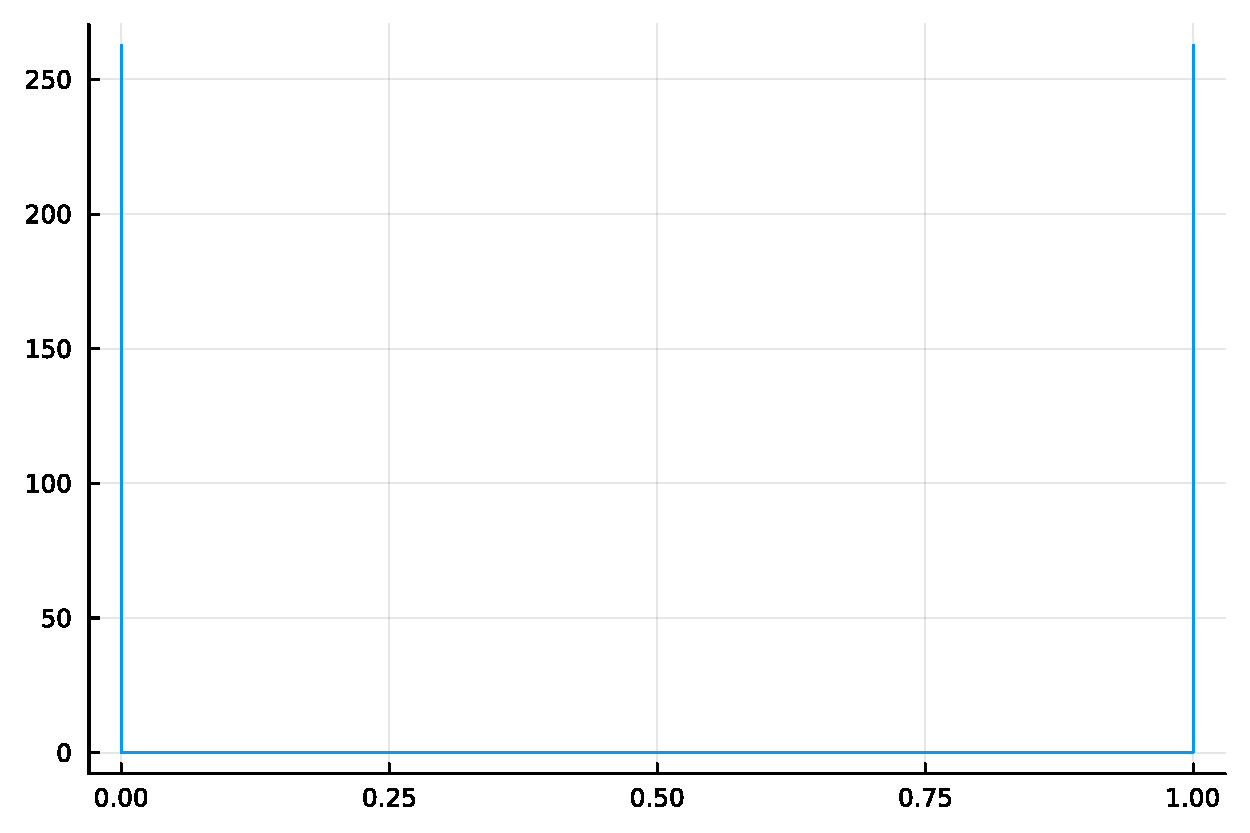
\includegraphics[width=0.3\linewidth]{experiments-fig/Ri1.pdf}}
%   % \quad
%   \subfigure[LTE.2]{
%     \label{fig:LTE2}
%     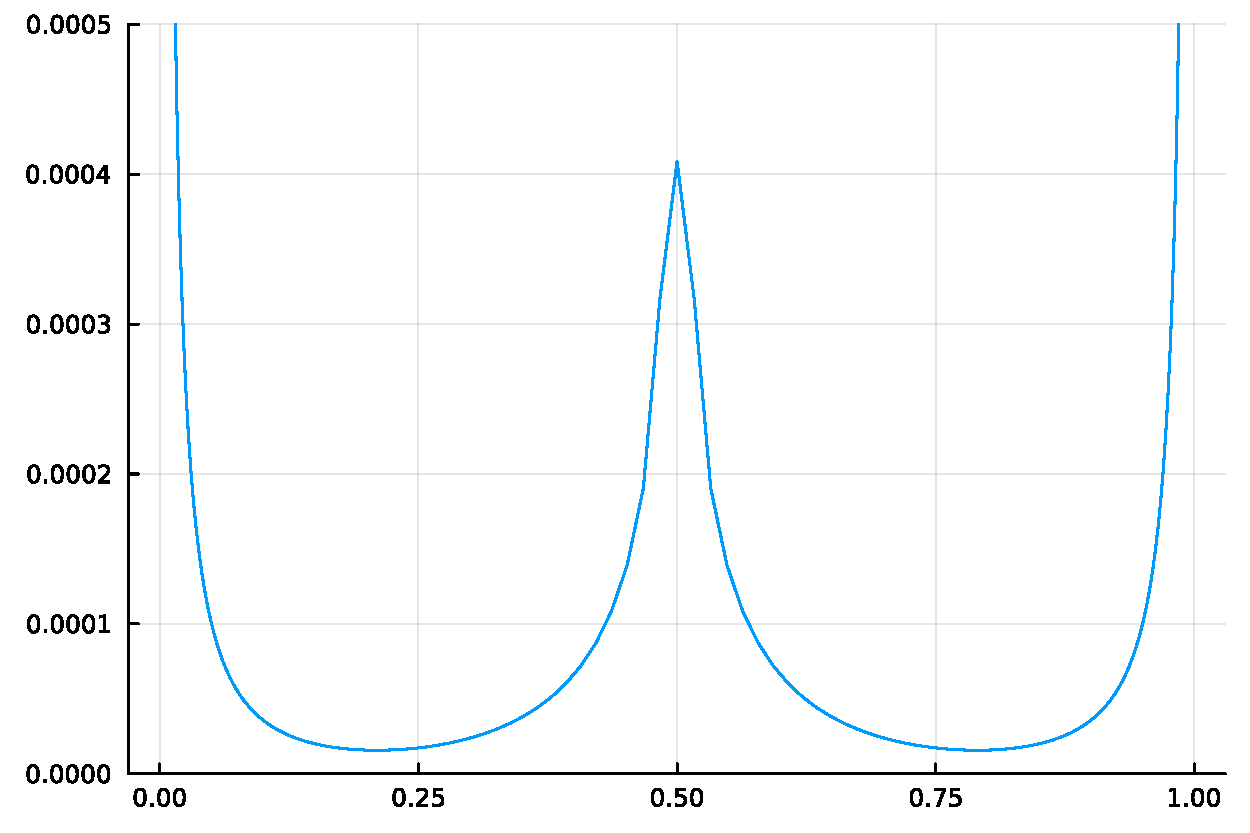
\includegraphics[width=0.3\linewidth]{experiments-fig/Ri2.pdf}}
%   % \quad
%   \subfigure[GE]{
%     \label{fig:GE}
%     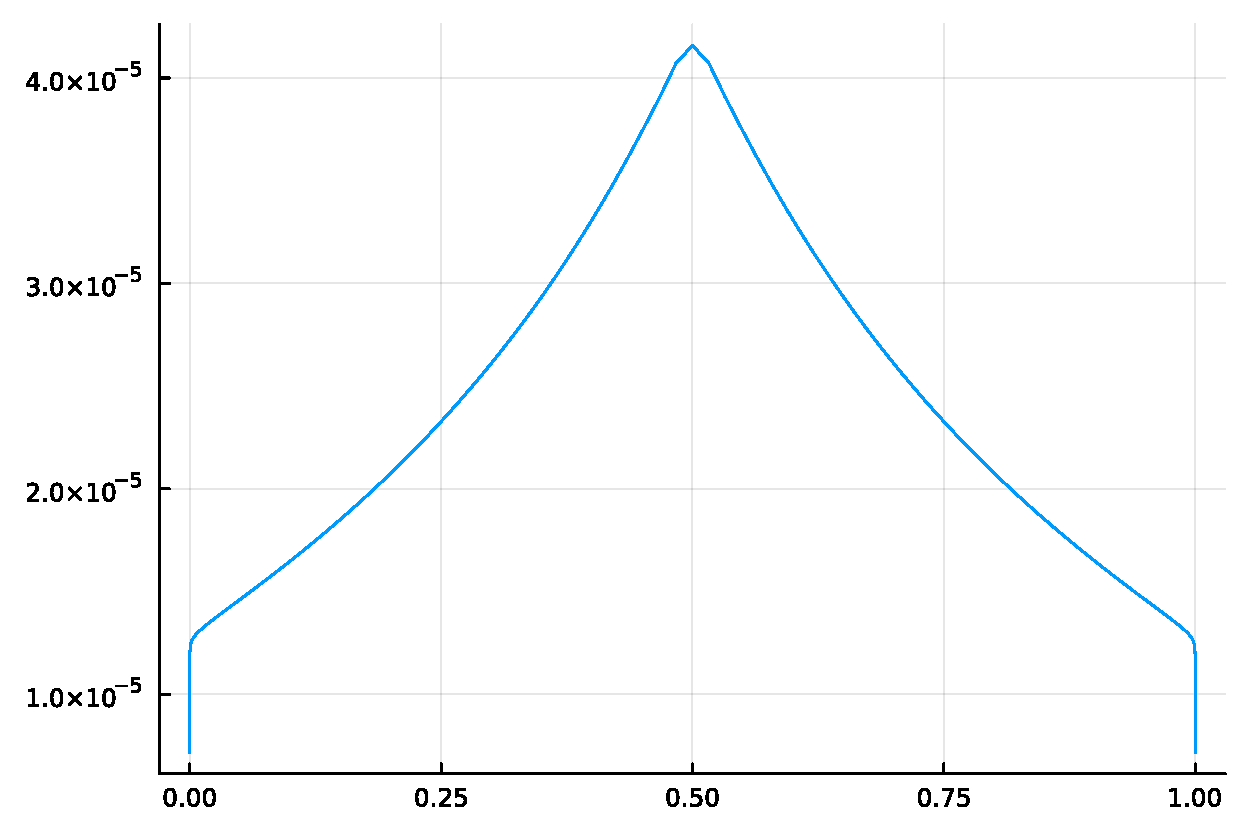
\includegraphics[width=0.3\linewidth]{experiments-fig/EN.pdf}}
%   \caption{truncation error and global error for \(f=1\), where \(\alpha=1.2\), \(r=4/\alpha\), \(2N=200\).}
% \end{figure}

% And \Cref{fig:LTE1} and \Cref{fig:LTE2} show the \(|\tau_i|\), whose difference is just ylim, and \Cref{fig:GE} shows the global error \(|u_i - u(x_i)|\).
% And that is the \Cref{fig:GE} suggests the technique we used in \Cref{subsec:proof-convergence}

\subsection{Singular source term}

% From \Cref{rmk:weak-reg-u}, 
We take the singular source term \(f(x)=x^{\sigma-\alpha}\), \(\sigma\in(0, \frac{\alpha}{2}]\) with $\sigma=0.4$ in \eqref{eq:equation}.
Since the analytic solution is unknown, the convergence rate of the numerical results is computed by
\begin{equation*}
  Rate^N = \log_2 \left( \frac{E^{N/2}}{E^{N}} \right)
  \quad \text{with} \quad
  E^N = \max_{0\le i\le N} |u^{N/2}_i - u^{N}_{2i}|.
\end{equation*}

% Let \(\sigma = 0.4\),


% , and take \(r=1, \frac{2}{\sigma}\) and various \(\alpha\), then display the values of \(E^N\) and \(Rate^N\) for various \(N\) in \Cref{tab:sig-r=1} and \Cref{tab:sigr2os}.
\begin{table}[htbp]
  \footnotesize
  \caption{\(r=1\):maximum nodal errors showing convergence rate $\mathcal{O}(h^{\sigma})$}\label{tab:sig-r=1}
  \begin{center}
    \begin{tabular}{|l|l|l|l|l|} \hline
      \diagbox{\(\alpha\)}{\(N\)} &  100 &  200 & 400 & 800 \\ 
      \hline
      1.2       & 2.9193e-2     & 2.2619e-2        & 1.7435e-2       & 1.3395e-2  \\
                &              & 0.3681         & 0.3755        & 0.3804    \\
      1.5       & 4.0497e-2      & 3.1068e-2        & 2.3717e-2       & 1.8057e-2  \\
                &              & 0.3824         & 0.3895        & 0.3934    \\
      1.8       & 5.6776e-2       & 4.3468e-2        & 3.3112e-2       & 2.5161e-2  \\
                &              & 0.3853         & 0.3926        & 0.3962    \\
      \hline
    \end{tabular}
  \end{center}
\end{table}
\begin{table}[htbp]
  \footnotesize
  \caption{\(r=\frac{2}{\sigma}\):maximum nodal errors showing convergence rate $\mathcal{O}(h^{2})$}\label{tab:sigr2os}
  \begin{center}
    \begin{tabular}{|l|l|l|l|l|} \hline
      \diagbox{\(\alpha\)}{\(2N\)} &  100 &  200 & 400 & 800\\ \hline
      1.2       & 2.7820e-3      & 6.9631e-4        & 1.7418e-4       & 4.3557e-5  \\
                &        & 1.9983   & 1.9992  & 1.9996    \\
      1.5       & 3.1742e-3      & 8.0150e-4        & 2.0223e-4       & 5.0947e-5  \\
                &        & 1.9856   & 1.9867  & 1.9889    \\
      1.8       & 5.0311e-3      & 1.3190e-3        & 3.4157e-4       & 8.7691e-5  \\ 
                &        & 1.9315   & 1.9492  & 1.9617    \\
      \hline
    \end{tabular}
  \end{center}
\end{table}

\Cref{tab:sig-r=1,tab:sigr2os} show that the difference-quadrature method \eqref{eq:equation_matrix} has convergence order
$\mathcal{O}(h^{\min \{r\sigma, 2\}})$, which agrees with \Cref{rmk:weak-reg-u}.



% \section{Conclusion}








\appendix

\section{Approximations of difference and interpolation}
In this appendix, we provide some approximations for the second-order difference quotients $D_h^2$ and the interpolation error $u(x)-\Pi_h u(x)$.
\begin{lemma} \label{lmm:Dh2simd2}
  Let $D_h^2$ be the difference quotient operator defined by \eqref{def:Dh2}.
  If \(g(x)\in C(\bar{\Omega}) \cap C^2(\Omega)\),
  there exists \(\xi\in (x_{i-1}, x_{i+1})\), $i=1, 2, ..., 2N-1$, such that
  \begin{equation*} \label{eq:Dh2simd2}
    \begin{aligned}
      D_h^2 g(x_i) & = g''(\xi), \quad \xi \in (x_{i-1}, x_{i+1}).
    \end{aligned}
  \end{equation*}
  % \begin{equation} \label{eq:Dh2Cauchy2}
  %   \begin{aligned}
  %      & \frac{2}{h_i + h_{i+1}} \left( \frac{1}{h_{i+1}} g(x_{i+1}) - (\frac{1}{h_{i}}+\frac{1}{h_{i+1}})g(x_{i}) + \frac{1}{h_{i}} g(x_{i-1}) \right)                          \\
  %     % &= \frac{h_i}{h_i + h_{i+1}} g''(\xi_1) + \frac{h_{i+1}}{h_i + h_{i+1}} g''(\xi_2)  \\
  %      & \quad = \frac{2}{h_i + h_{i+1}} \left( \frac{1}{h_{i}}\int_{x_{i-1}}^{x_i} g''(y) (y-x_{i-1}) dy + \frac{1}{h_{i+1}} \int_{x_i}^{x_{i+1}} g''(y) (x_{i+1}-y) dy \right)
  %   \end{aligned}
  % \end{equation}
  Moreover, if \(g(x) \in C(\bar{\Omega}) \cap C^4(\Omega)\), then we have
  \begin{equation*} \label{eq:Dh2simd4}
    \begin{aligned}
      & D_h^2 g(x_i) = g''(x_{i}) + \frac{h_{i+1}-h_{i}}{3} g'''(x_{i}) \\
      &  +  \frac{2}{h_i + h_{i+1}}\left( \frac{1}{h_{i}}\int_{x_{i-1}}^{x_i} g''''(y) \frac{(y-x_{i-1})^3}{3!} dy + \frac{1}{h_{i+1}} \int_{x_i}^{x_{i+1}} g''''(y) \frac{(x_{i+1}-y)^3}{3!} dy \right) .
    \end{aligned}
  \end{equation*}
\end{lemma}
\begin{proof}
  By Taylor series expansion, we obtain
  \begin{gather*}
    g(x_{i-1}) = g(x_{i}) - (x_{i}-x_{i-1}) g'(x_{i}) + \frac{(x_{i}-x_{i-1})^2}{2} g''(\xi_1), \quad \xi_1 \in (x_{i-1}, x_{i}),        \\
    g(x_{i+1}) = g(x_{i}) + (x_{i+1}-x_{i}) g'(x_{i}) + \frac{(x_{i+1}-x_{i})^2}{2} g''(\xi_2), \quad \xi_2 \in (x_{i}, x_{i+1}).
  \end{gather*}
  From \eqref{def:Dh2} and the above equations, it yields
  \begin{equation*}
    \begin{aligned}
      D_h^2 g(x_i) & = \frac{2}{h_i + h_{i+1}} \left( \frac{1}{h_{i+1}} \left(g(x_{i+1})-g(x_i)\right)  + \frac{1}{h_{i}} \left(g(x_{i-1})-g(x_i)\right) \right) \\
      &= \frac{h_i}{h_i + h_{i+1}} g''(\xi_1) + \frac{h_{i+1}}{h_i + h_{i+1}} g''(\xi_2)  .
    \end{aligned}
  \end{equation*}
  According to intermediate value theorem, there exists some \(\xi \in [\xi_1, \xi_2]\) such that
  \begin{equation*}
    D_h^2 g(x_i) = \frac{h_i}{h_i + h_{i+1}} g''(\xi_1) + \frac{h_{i+1}}{h_i + h_{i+1}} g''(\xi_2) = g''(\xi).
  \end{equation*}
  % For the second equation, similarly
  % \begin{gather*}
  %   g(x_{i-1}) = g(x_{i}) - (x_{i}-x_{i-1}) g'(x_{i}) + \int_{x_{i-1}}^{x_i} g''(y) (y-x_{i-1}) dy \\
  %   g(x_{i+1}) = g(x_{i}) + (x_{i+1}-x_{i}) g'(x_{i}) + \int_{x_i}^{x_{i+1}} g''(y) (x_{i+1}-y) dy
  % \end{gather*}
  % The second equation can be also obtained by Taylor expansion similarly.
  The second equation can also be derived in a similar manner through Taylor expansion. 
  The proof is completed.
  % \begin{gather*}
  %   g(x_{i-1}) = g(x_{i}) - h_{i} g'(x_{i}) + \frac{h_{i}^2}{2} g''(x_{i}) - \frac{h_{i}^3}{3!} g'''(x_{i}) +  \int_{x_{i-1}}^{x_{i}} g''''(y) \frac{(y-x_{i-1})^3}{3!} dy  ,      \\
  %   g(x_{i+1}) = g(x_{i}) + h_{i+1} g'(x_{i}) + \frac{h_{i+1}^2}{2} g''(x_{i}) + \frac{h_{i+1}^3}{3!} g'''(x_{i}) + \int_{x_{i}}^{x_{i+1}} g''''(y) \frac{(x_{i+1}-y)^3}{3!} dy .
  % \end{gather*}
  % In particular,
  % \begin{equation} \label{eq:Dh2Cauchy4}
  %   \begin{aligned}
  %     \int_{x_{i-1}}^{x_{i}} g''''(y) \frac{(y-x_{i-1})^3}{3!} dy & = \frac{h_i^4}{4!}g''''(\eta_1) \\
  %     \int_{x_{i}}^{x_{i+1}} g''''(y) \frac{(x_{i+1}-y)^3}{3!} dy & = \frac{h_{i+1}^4}{4!}g''''(\eta_2)
  %   \end{aligned}
  % \end{equation}
  % where \(\eta_1 \in (x_{i-1}, x_{i}), \eta_2 \in (x_{i}, x_{i+1})\).
\end{proof}


\begin{lemma} \label{lmm:Dyj}
  Let \(y_j^\theta = (1-\theta) x_{j-1} + \theta x_j, \theta\in (0,1)\) with $2\le j\le 2N-1$. Then we have
  % then for \(2\le j \le 2N-1\)
  \begin{equation*}
    \begin{aligned}
      u(y_j^\theta) - \Pi_hu(y_j^\theta) & = -\frac{\theta (1-\theta)}{2} h_j^2 u''(\xi), \quad \xi \in (x_{j-1}, x_j),
    \end{aligned}
  \end{equation*}
  and
  \begin{equation*}
    \begin{aligned}
      u(y_j^\theta) - \Pi_hu(y_j^\theta) = & -\frac{\theta (1-\theta)}{2} h_j^2 u''(y_j^\theta)
      + \frac{\theta (1-\theta)}{3!} h_j^3 \left(\theta^2 u'''(\eta_1) - (1-\theta)^2 u'''(\eta_2) \right)
    \end{aligned}
  \end{equation*}
  with \(\eta_1 \in (x_{j-1}, y_j^\theta), \eta_2 \in (y_j^\theta, x_j)\).
\end{lemma}
\begin{proof}
  Using Taylor series expansion, we get
  \begin{gather*}
    u(x_{j-1}) = u(y_j^\theta) - \theta h_{j} u'(y_j^\theta) + \frac{\theta^2 h_{j}^2}{2!} u''(\xi_1), \quad \xi_1 \in (x_{j-1}, y_j^\theta) ,\\
    u(x_{j}) = u(y_j^\theta) + (1-\theta) h_{j} u'(y_j^\theta) + \frac{(1-\theta)^2 h_{j}^2}{2!} u''(\xi_2) , \quad \xi_2 \in (y_j^\theta, x_j) ,
  \end{gather*}
  which implies that
  \begin{equation*}
    \begin{aligned}
      u(y_j^\theta) - \Pi_hu(y_j^\theta) 
      & = u(y_j^\theta) - (1-\theta) u(x_{j-1}) - \theta u(x_{j})      \\
      & = -\frac{\theta (1-\theta)}{2} h_j^2 ( \theta u''(\xi_1) + (1-\theta) u''(\xi_2) ) \\
      & = -\frac{\theta (1-\theta)}{2} h_j^2 u''(\xi), \quad \xi \in [\xi_1, \xi_2].
    \end{aligned}
  \end{equation*}
  The second equation can be similarly obtained by
  \begin{gather*}
    u(x_{j-1}) = u(y_j^\theta) - \theta h_{j} u'(y_j^\theta) + \frac{ \theta^2h_{j}^2}{2!} u''(y_j^\theta) - \frac{\theta^3 h_{j}^3}{3!} u'''(\eta_1) , \\
    u(x_{j}) = u(y_j^\theta) + (1-\theta) h_{j} u'(y_j^\theta) + \frac{(1-\theta)^2 h_{j}^2}{2!} u''(y_j^\theta) + \frac{(1-\theta)^3 h_{j}^3}{3!} u'''(\eta_2) 
  \end{gather*}
  with \(\eta_1 \in (x_{j-1}, y_j^\theta), \eta_2 \in (y_j^\theta, x_j)\).
  % And
  % \begin{equation*}
  %   \begin{aligned}
  %     u(y_j^\theta) - \Pi_hu(y_j^\theta) 
  %     & = u(y_j^\theta) - (1-\theta) u(x_{j-1}) -\theta u(x_{j})   .
  %     % & = -\frac{\theta (1-\theta)}{2} h_j^2 u''(y_j^\theta) + \frac{\theta (1-\theta)}{3!} h_j^3 ( \theta^2 u'''(\eta_1) - (1-\theta)^2 u'''(\eta_2))
  %   \end{aligned}
  % \end{equation*}
  The proof is completed.
\end{proof}

\begin{lemma} \label{lmm:Dyjleh2ya/2m2/r}
  For any $y\in (x_{j-1}, x_{j})$, \(2\le j \le 2N-1\), there exists 
  \begin{equation*}
    |u(y)-\Pi_hu(y)| \le h_j^2 \max_{\xi\in [x_{j-1}, x_j]}|u''(\xi)| \le C h^2 \delta(y)^{\alpha/2-2/r}.
  \end{equation*}
\end{lemma}
\begin{proof}
  According to \Cref{lmm:Dyj,lmm:regularity-u,lmm:hilexi}, the desired result is obtained.
\end{proof}

\begin{lemma} \label{lmm:Dyj1}
  For any \(x\in [x_{j-1}, x_j]\), $1\le j \le 2N$, there exists
  \begin{equation*}
    \begin{aligned}
      |u(x) - \Pi_hu(x)| & =\! \left| \frac{x_{j}-x}{h_j} \int_{x_{j-1}}^x u'(y) dy - \frac{x-x_{j-1}}{h_j} \int_{x}^{x_{j}} u'(y) dy \right| 
                       \le \!\int_{x_{j-1}}^{x_{j}} |u'(y)| dy.
    \end{aligned}
  \end{equation*}
  In particular, there exist,
  % If \(x\in [0, x_1]\), %with \Cref{lmm:regularity-u}, we have
  \begin{equation*}
    |u(x) - \Pi_hu(x)| \le 
    % \int_{0}^{x_1} |u'(y)| dy \le \int_{0}^{x_1} C y^{\alpha/2-1} dy  \le C\frac{2}{\alpha} x_1^{\alpha/2} = 
    C\frac{2}{\alpha} h_1^{\alpha/2}, \quad x\in (0, x_1) \cup (x_{2N-1}, 2T).
  \end{equation*}
  % Similarly, if \(x\in [x_{2N-1}, 2T]\), there exist
  % \begin{equation*}
  %   |u(x) - \Pi_hu(x)| \le C\frac{2}{\alpha} (2T-x_{2N-1})^{\alpha/2} = C\frac{2}{\alpha} h_{2N}^{\alpha/2} .
  % \end{equation*}
\end{lemma}
\begin{proof}
    From the definition of $\Pi_h u(x)$ in \eqref{def:interp} and using $u(x) = u(x_i) + \int_{x_i}^{x} u'(y) dy$, the proof is completed.
\end{proof}





\section{Bound estimates}
Set
\(
  h_i = x_{i} - x_{i-1}
\) for $j = 1, 2, ... ,  2N$ 
and define $h := \frac{1}{N}$. 
The following bounds are needed in several places.
% and the definition of \(\simeq\) in \Cref{sec:numformat}
\begin{lemma} \label{lmm:hi1-hi}
For \(i=1,2,\cdots,2N-1\), there exists a constant \(C\) such that 
\begin{equation*}
  |h_{i+1} - h_{i}| \le C(r-1) h^2 \delta(x_i)^{1-2/r} , \quad r\ge 1.
\end{equation*}
\end{lemma}
\begin{proof}
According to the definition of $h_i=x_i-x_{i-1}$ as defined in \eqref{def:xj}, we obtain
\begin{equation*}
  \begin{aligned}
    h_{i+1} - h_{i} =
    \begin{cases}
      T \left( \left(\frac{i+1}{N}\right)^r - 2\left(\frac{i}{N}\right)^r + \left(\frac{i-1}{N}\right)^r  \right) ,           & 1\le i\le N-1,    \\
      0,    & i=N,    \\
      -T \left( \left(\frac{2N-i-1}{N}\right)^r - 2\left(\frac{2N-i}{N}\right)^r + \left(\frac{2N-i+1}{N}\right)^r  \right) , & N+1\le i\le 2N-1 .    \\
    \end{cases}
  \end{aligned}
\end{equation*}
Since $(i+1)^r - 2i^r + (i-1)^r \simeq r(r-1)i^{r-2}$ for $i\ge 1$,
the desired result is obtained.
\end{proof}




\begin{lemma} \label{lmm:trucerr2d2f}
For $1\le i \le 2N-1$,
  there exists a constant \(C\) such that
    \begin{equation*}
      \begin{aligned}
        & \frac{2}{h_i + h_{i+1}} \left| \frac{1}{h_i} \int_{x_{i-1}}^{x_{i}} f''(y) \frac{(y-x_{i-1})^3}{3!} dy + \frac{1}{h_{i+1}} \int_{x_{i}}^{x_{i+1}} f''(y) \frac{(y-x_{i+1})^3}{3!} dy \right| \\
         & \quad \le C h^2 \delta(x_i)^{-\alpha/2-2/r} .
      \end{aligned}
    \end{equation*}
\end{lemma}
\begin{proof} \label{prf:trucerr2d2f}
  By \Cref{lmm:regularity-u}, for \(1 \le i \le 2N-1\), we have
  \begin{equation*}
    \begin{aligned}
      \left|\int_{x_{i-1}}^{x_{i}} f''(y)\frac{(y-x_{i-1})^3}{3!} dy \right|  \le \frac{\|f\|_{\beta}^{(\alpha/2)}}{3!} \int_{x_{i-1}}^{x_{i}} \delta(y)^{-\alpha/2-2} (y-x_{i-1})^3 dy .
    \end{aligned}
  \end{equation*}
  For \(i=1\), we get
  \begin{equation*}
    \int_{x_{i-1}}^{x_{i}} \delta(y)^{-\alpha/2-2} (y-x_{i-1})^3 dy
    = \int_{0}^{x_{1}} y^{1-\alpha/2} dy
    = \frac{1}{2-\alpha/2} x_1^{2-\alpha/2} \simeq x_1^{-\alpha/2-2} h_1^4 .
  \end{equation*}
  For \(2\le i \le 2N-1\), by \Cref{lmm:hilexi}, we have
  \begin{equation*}
    \begin{aligned}
      \int_{x_{i-1}}^{x_{i}} \delta(y)^{-\alpha/2-2} (y-x_{i-1})^3 dy 
        \simeq \int_{x_{i-1}}^{x_{i}} \delta(x_i)^{-\alpha/2-2} (y-x_{i-1})^3 dy
        \simeq \delta(x_i)^{-\alpha/2-2} h_i^4
    \end{aligned}
  \end{equation*}
  % Thus, for  \(1\le i\le 2N-1\), we have 
  % \begin{equation*}
  %   \left|\int_{x_{i-1}}^{x_{i}} f''(y)\frac{(y-x_{i-1})^3}{3!} dy \right| \le C \delta(x_i)^{-\alpha/2-2} h_i^4 .
  % \end{equation*}
  % The following estimation can be checked similarly
  % \begin{equation*}
  %   \left|\int_{x_{i}}^{x_{i+1}} f''(y)\frac{(x_{i+1}-y)^3}{3!} dy \right| \le C \delta(x_i)^{-\alpha/2-2} h_{i+1}^4 .
  % \end{equation*}
  % Thus for \(1\le i\le 2N-1\), with \Cref{lmm:hilexi} we have
  % \begin{equation*}
  %   \begin{aligned}
  %     & \frac{2}{h_i + h_{i+1}} \left| \frac{1}{h_i} \int_{x_{i-1}}^{x_{i}} f''(y) \frac{(y-x_{i-1})^3}{3!} dy 
  %     % + \frac{1}{h_{i+1}} \int_{x_{i}}^{x_{i+1}} f''(y) \frac{(y-x_{i+1})^3}{3!} dy 
  %     \right| \\
  %      & \quad \le C \delta(x_i)^{-\alpha/2-2} \frac{h_i^3}{h_i + h_{i+1}} 
  %      \simeq \delta(x_i)^{-\alpha/2-2} h_i^2 \simeq  h^2 \delta(x_i)^{-\alpha/2-2/r}.
  %   \end{aligned}
  % \end{equation*}
  % It's symmetric for \(N < i \le 2N-1\).
  The desired result is obtained.
\end{proof}

\begin{lemma} \label{lmm:Dh2Kyxi}
  For all \(1 \le i \le 2N-1\), \(1\le j \le 2N\), $y\in (x_{j-1}, x_{j})$, there exist
  % s.t. \(\min\{|j-i|, |j-1-i|\} \ge 2\) and \(y\in [x_{j-1}, x_{j}]\), we have
  \begin{gather*}
    |D_h K_y (x_i)| \simeq | x_i - y|^{-\alpha} \quad\text{if}\quad [x_{j-1}, x_{j}] \cap [x_i, x_{i+1}] = \varnothing , \\
    D_h^2 K_y (x_i) \simeq | x_i - y |^{-1-\alpha} \quad\text{if}\quad [x_{j-1}, x_{j}] \cap [x_{i-1}, x_{i+1}] = \varnothing.
  \end{gather*}
\end{lemma}
\begin{proof}
  Since \(x_{i-1}-y\), \(x_{i}-y\) and \(x_{i+1}-y\) have the same sign, using \Cref{lmm:Dh2simd2} and $K_y(x) = \frac{\kappa_\alpha}{\Gamma(2-\alpha)}|x-y|^{1-\alpha}$ in \eqref{def:Kyx}, it yields
  \begin{equation*}
    \begin{aligned}
      |D_h K_y (x_i)| &= \frac{\kappa_\alpha(\alpha-1)}{\Gamma(2-\alpha)}|\xi-y|^{-\alpha}, \quad \xi\in (x_{i}, x_{i+1})  ,\\
      D_h^2 K_y (x_i) & = \frac{\kappa_\alpha \alpha(\alpha-1)}{\Gamma(2-\alpha)}|\xi-y|^{-1-\alpha}, \quad \xi\in (x_{i-1}, x_{i+1})  .
    \end{aligned}
  \end{equation*}
  Moreover, from \(|\xi-y| \simeq |x_i-y|\), the desired result is obtained.
\end{proof}


\begin{lemma} \label{lmm:sumSij13}
  There exists a constant $C$ such that
  \begin{gather*}
    \sum_{j=1}^{3} V_{1j} \le C h^2 x_1^{-\alpha/2-2/r}  \quad \text{and} \quad
    \sum_{j=1}^{4} V_{2j} \le C h^2 x_2^{-\alpha/2-2/r}  .
  \end{gather*}
\end{lemma}
\begin{proof}
  According \Cref{lmm:Dyj1}, \Cref{lmm:Dyjleh2ya/2m2/r}, \eqref{def:Tij}, \eqref{def:Vij}, it implies, 
  \begin{equation*}
    T_{ij} \le C x_1^{2-\alpha/2} \simeq h_1^2 \; h^2 x_1^{-\alpha/2-2/r} \simeq h_1^2 \; h^2 x_2^{-\alpha/2-2/r} \quad \text{for}\quad 0\le i \le 3, 1\le j \le 4.
  \end{equation*}
  The proof is completed.
\end{proof}

\begin{lemma} \label{ineq:a-b-theta}
Let $a,b> 0,\; \theta \in [0,1]$. Then we have
  \begin{equation*}
    b^{1-\theta}|a^{\theta}-b^{\theta}| \le |a-b|. %\; (\text{  also  }a^{1-\theta}|a^{\theta}-b^{\theta}| \le |a-b|).
  \end{equation*}
\end{lemma}
\begin{proof}
    Since $|t^\theta - 1| \le |t-1|$ with $t=\frac{a}{b} > 0$, the proof is completed.
\end{proof}


\begin{lemma} \label{eq:ineq_fxy}
    Let $x > 0, y\ge 1$ with $\alpha \in (1,2)$. Then we have
    \begin{equation*}
        \begin{aligned}
    f(x,y) =& xy(1+x^{2-\alpha} +y^{2-\alpha}) + (1+x+y)^{3-\alpha} \\
         &- (1+x)(1+y)\left( (1+x)^{2-\alpha} + (1+y)^{2-\alpha} - 1 \right) > 0.
        \end{aligned}
    \end{equation*}
\end{lemma}
\begin{proof}
    % It is obvious that $f(x,y)=f(y,x)$ and $f(0, y) = f(x, 0) = 0$. 
    The first and second derivatives of $f(x,y)$ with respect to $x$ are
    \begin{gather*}
        \begin{aligned}
        \partial_x f(x,y) =&  
            (3-\alpha)\left[ x^{2-\alpha} y + (1+x+y)^{2-\alpha} - (1+x)^{2-\alpha}(1+y) \right] \\
            &+ 1+2y+y^{3-\alpha}-(1+y)^{3-\alpha} ,
        \end{aligned}  \\
        \partial_x^2 f(x, y) = (3-\alpha)(2-\alpha) \left( y x^{1-\alpha} + (1+x+y)^{1-\alpha} - (1+y) (1+x)^{1-\alpha} \right).
    \end{gather*}
    Since $\frac{y}{1+y}x + \frac{1}{1+y}(1+x+y) = 1+x$
    and $x^{1-\alpha}$ is convex for $x>0$,
    using Jensen's inequality, it yields
    \begin{equation*}
        \frac{y}{1+y} x^{1-\alpha} + \frac{1}{1+y} (1+x+y)^{1-\alpha} > (1+x)^{1-\alpha},
    \end{equation*}
    which implies $\partial_x^2 f(x, y) > 0$ and $\partial_x f(x, y)>\partial_x f(0, y)$. % and $\partial_y^2 f(x, y) > 0$.

    Since $\partial_x f(0, y)>0$ for $y\ge 1$, we have $f(x,y)>f(0,y)=0$.
    The proof is completed.
    
    % Since $f(x, 0) = 0$, it is sufficient to prove $f(x,1) > 0$. 
    % While $f(0, 1) = 0$ and $\partial_x^2 f(x, 1) > 0$, we only need to prove that $\partial_x f(0, 1) > 0$, where
    % \begin{equation*}
    %     \partial_x f(0, 1) = 4 - 2(3-\alpha) - (\alpha-1) 2^{2-\alpha} > 0.
    % \end{equation*}
    % The proof is completed.
\end{proof}





\section{Proofs for grid mapping functions}
\label{sec:prfs-of-GMFs}
In this appendix, we provide the proofs of Lemmas \ref{lmm:gen-prop-of-MTFs}-\ref{lmm:dQj-itle} in \cref{subsec:mesh-transport-functions}.
\begin{proof} [\bf Proof of \Cref{lmm:gen-prop-of-MTFs}]
  \label{prf:gen-prop-of-MTFs}
  The first two approximations can be derived from \eqref{def:xj} and \eqref{eq:prop-of-GMFs} with $2\le i, j \le 2N-2$.    \par
  We next prove $|y_{i,j}(\xi) - \xi| \simeq |x_j - x_i|$.
  From \eqref{def:yij}, we have $y_{i,j}(\xi)-\xi = 0$ if $i=j$. 
  Without loss of generality, if $i< j$, then $ y_{i,j}(\xi) - \xi \le x_{j+1} - x_{i-1} \simeq x_j - x_i$.
  Since the second derivatives of $|y_{i,j}(\xi) - \xi|$ is less than zero by \Cref{lmm:derivatives-of-MTFs}, which implies it is concave. Thus, $|y_{i,j}(\xi) - \xi| \ge \min\{x_{j-1}-x_{i-1}, x_{j+1}-x_{i+1}\} \simeq |x_{j} - x_{i}| $.  \par
  From \eqref{def:yij}, \eqref{def:hij}, \eqref{eq:prop-of-GMFs}, using the approximation above, there exists
  $$ h_{i,j}(\xi) = y_{i,j}(\xi) - y_{i,j-1}(\xi) = y_{j-1, j}(y_{i,j-1}(\xi)) - y_{i,j-1}(\xi) \simeq x_{j} - x_{j-1}=h_j. $$
  
  The final estimate can be obtained since \(y_{i,j-1}(\xi) - \xi\), \(y_{i,j}(\xi) - \xi\) have the same sign \((\ge 0\) or \(\le 0)\).
\end{proof}


\begin{proof} [\bf Proof of \Cref{lmm:esitmate-of-MTFs-1}]
  From \eqref{def:hij} and \Cref{lmm:derivatives-of-MTFs}, we can see that
  \begin{equation*}
    \begin{aligned}
      & h_{i,j}'(x) = y_{i,j}'(x) - y_{i,j-1}'(x) \\ 
      &=\begin{cases}
        x^{1/r-1} \left( y_{i,j}^{1-1/r}(x) - y_{i,j-1}^{1-1/r}(x) \right) ,& i< N, j< N, \\
        x^{1/r-1} \left( \dfrac{h_N}{r Z_1} - y_{i,N-1}^{1-1/r}(x) \right)  ,& i< N, j=N, \\
        x^{1/r-1} \left( (2T-y_{i,N+1}(x))^{1-1/r} - \dfrac{h_N}{r Z_1}  \right)   ,& i< N, j=N+1, \\
        x^{1/r-1} \left( (2T-y_{i,j}(x))^{1-1/r} - (2T-y_{i,j-1}(x))^{1-1/r} \right)   ,& i< N, j>N+1, \\
        \dfrac{rZ_1}{h_N} \left( y_{N,j}^{1-1/r}(x) - y_{N,j-1}^{1-1/r}(x) \right)  ,& i=N, j< N ,\\
        \dfrac{rZ_1}{h_N} \left( \dfrac{h_N}{rZ_1} - y_{N,N-1}^{1-1/r}(x) \right)   ,& i=N, j=N .
      \end{cases}
    \end{aligned}
  \end{equation*}
  
  For \(2\le i\le N\), \(2\le j < N\), it yields%\(\xi \in (x_{i-1}, x_{i+1})\),
  \begin{equation} \label{eq:yij1-1/r-j-1}
    \begin{aligned}
      y_{i,j}^{1-1/r}(\xi) - y_{i,j-1}^{1-1/r}(\xi)
      &\le x_{j+1}^{1-1/r} - x_{j-2}^{1-1/r}  \\
      &= T^{1-1/r} N^{1-r} \left( (j+1)^{r-1} - (j-2)^{r-1} \right) \\
      & \le C T^{1-1/r} (r-1) N^{1-r} j^{r-2} = C  (r-1) Z_1 x_j^{1-2/r}.
    \end{aligned}
  \end{equation}
  % and similar for \(N+1 < j \le 2N-1\).
  
  For $2\le i\le N$, \(j=N\), since %we have \(y_{i,N-1}(\xi) \in (x_{N-2}, x_{N})\).
  \begin{equation} \label{eq:hN/rZ1}
    \dfrac{h_N}{r Z_1} = T^{1-1/r} \dfrac{1 - (1-h)^r}{rh} = \eta^{1-1/r} \simeq x_N^{1-1/r}, \quad \eta \in (x_{N-1}, x_{N}),
  \end{equation}
  we have
  \begin{equation*} \label{eq:hN/rZ1-yj=N-1}
    |\dfrac{h_N}{r Z_1} - y_{i,N-1}^{1-1/r}(\xi)| \le x_N^{1-1/r} - x_{N-2}^{1-1/r} \simeq (r-1) Z_1 x_N^{1-2/r}.
  \end{equation*}
  
  For $2\le i\le N$, \(N+1\le j \le 2N-2\), it can be checked 
  $$|h_{i,j}'(\xi)| \le C (r-1)Z_1 \xi^{1/r-1} (2T-x_j)^{1-2/r}.$$
  Combine with \Cref{lmm:hilexi,lmm:gen-prop-of-MTFs}, the first inequality is obtained.

  On the other hand, from \eqref{def:yij}, we have $|y_{i,j}(x)-x| = \text{sign}(j-i) (y_{i,j}(x) - x)$ and $(y_{i,j}(x) - x)' = y_{i,j}'(x) - 1$.
  
  For \(2\le i < N\), \(2\le j<N\), by \Cref{ineq:a-b-theta,lmm:gen-prop-of-MTFs}, we have
  \begin{equation*}
    \xi^{1/r} |y_{i,j}^{1-1/r}(\xi) - \xi^{1-1/r}| \le |y_{i,j}(\xi) - \xi| \simeq |x_{j}-x_{i}|  .
  \end{equation*}
  
  For \(2\le i < N\), \(j=N\), using \eqref{eq:hN/rZ1} and \Cref{ineq:a-b-theta}, it yields
  \begin{equation} \label{eq:hN/rZ1-xi<N}
    \begin{aligned}
      \eta^{1/r} |\dfrac{h_N}{r Z_1} - \xi^{1-1/r}| &\le |\eta - \xi|, \quad \eta \in (x_{N-1}, x_{N})  \\
      & \le |x_N - x_i| + |h_N| + |h_{i+1}| \le 3 |x_N - x_i|.
    \end{aligned}
  \end{equation}
  
  For \(2\le i < N\), \(N<j\le 2N-2\), from \Cref{ineq:a-b-theta}, one has
  \begin{equation*} \label{eq:2T-yij1-1/r}
    \begin{aligned}
      &\xi^{1/r} |(2T-y_{i,j}(\xi))^{1-1/r} - \xi^{1-1/r}|
              \le |2T - y_{i,j}(\xi) - \xi|  \\
      & \quad \le |2T - x_j - x_i| + |y_{i,j}(\xi) - x_j| + |\xi - x_i|
              \le |2T - x_j - x_i| + 2 h_N   \\
      & \quad \le |x_j - T| + |T-x_i| + 2h_N \le 2 |x_j - x_i|.
    \end{aligned}
  \end{equation*}

  Similar to proof of \eqref{eq:hN/rZ1-xi<N}, we have
  \begin{equation*}
  \begin{gathered}
    \eta^{1/r} |y_{N, j}^{1-1/r}(\xi) - \dfrac{h_N}{r Z_1}| \le C |x_j - x_N|, \quad i=N, j<N, \\
    \eta^{1/r} |(2T-y_{N, j}(\xi))^{1-1/r} - \frac{h_N}{r Z_1}| \le C |x_j - x_N|, \quad i=N, j>N,
  \end{gathered}
  \end{equation*}
  and \(y_{N,N}(x) - x \equiv 0\).

  Thus, using \Cref{lmm:derivatives-of-MTFs,lmm:gen-prop-of-MTFs}, the second inequality is obtained.
\end{proof}



\begin{proof} [\bf Proof of \Cref{lmm:esitmate-of-MTFs-2}]
  By \Cref{def:gridmapfunc}, \Cref{ineq:a-b-theta} and \eqref{eq:hN/rZ1}, there exist
  \begin{equation} \label{eq:Zj-i}
  \begin{split}
    &x_j^{1-1/r} |Z_{j-i}| = x_j^{1-1/r} |x_j^{1/r} - x_i^{1/r}| \le |x_j - x_i|, \quad i<N, j < N, \\
    &Z_{2N-j+i} \le Z_{2N} =  2 T^{1/r},                    \qquad i<N, j>N,    \\
    &\dfrac{h_N}{r Z_1} \simeq x_N^{1-1/r},      \qquad i=N, 2\le j \le 2N-2. 
  \end{split}
  \end{equation}
  Combine with \Cref{lmm:derivatives-of-MTFs,lmm:gen-prop-of-MTFs}, the first inequality is obtained.

  From \eqref{def:hij}, it yields $h_{i,j}''(x) = y_{i,j}''(x) - y_{i,j-1}''(x)$.
  For $3\le j \le 2N-2$, we have
  \begin{equation}   \label{eq:y1-2/r}
  \begin{gathered}
  |y_{i,j}^{1-2/r}(\xi) - y_{i,j-1}^{1-2/r}(\xi)| \simeq (r-2) Z_1 x_j^{1-3/r},  \\
  |(2T-y_{i,j}(\xi))^{1-2/r} - (2T-y_{i,j-1}(\xi))^{1-2/r}| \simeq (r-2) Z_1 (2T-x_j)^{1-3/r},  \\
  \end{gathered}
  \end{equation}
  which can be similarly proven as \eqref{eq:yij1-1/r-j-1}. 
    
  For \(2\le i<N\), \(3\le j<N\), it yields
  \begin{equation*} \label{eq:yij1-2/rZj-i-depart}
    \begin{aligned}
      y_{i,j}^{1-2/r}(\xi) Z_{j-i} - y_{i,j-1}^{1-2/r}(\xi) Z_{j-i-1}
      = \left( y_{i,j}^{1-2/r}(\xi) - y_{i,j-1}^{1-2/r}(\xi) \right) Z_{j-i} + y_{i, j-1}^{1-2/r}(\xi) Z_1.
    \end{aligned}
  \end{equation*}
  Combine with \eqref{eq:Zj-i} and \eqref{eq:y1-2/r}, we get
  \begin{equation*} \label{eq:yij1-2/rZj-i-}
    |y_{i,j}^{1-2/r}(\xi) Z_{j-i} - y_{i,j-1}^{1-2/r}(\xi) Z_{j-i-1}| \le C Z_1 \left( |r-2| x_j^{-2/r}|x_j - x_i| + x_j^{1-2/r}  \right).
  \end{equation*}
  
  For $2\le i < N$, \(j=N, N+1\), it leads to
      $$|h_{i,j}''(x)| \le |y_{i,j}''(x)| + |y_{i,j-1}''(x)| \le C (r-1) x_i^{1/r-2} x_N^{1-1/r}.$$


  For $2\le i<N$, \(j > N+1\), from \Cref{lmm:hilexi} and \eqref{eq:y1-2/r}, we have
  \begin{equation*}
    \begin{aligned}
      & \left|  \delta(y_{i,j}(\xi))^{1-2/r} Z_{2N-(j-i)} - \delta(y_{i,j-1}(\xi))^{1-2/r} Z_{2N-(j-i-1)}  \right| \\
      & = \left|  \left( \delta(y_{i,j}(\xi))^{1-2/r} - \delta(y_{i,j-1}(\xi))^{1-2/r} \right) Z_{2N-(j-i)} - \delta(y_{i, j-1}(\xi))^{1-2/r} Z_1  \right|   \\
      % &\left|(2T-y_{i,j}(\xi))^{1-2/r} Z_{2N-(j-i)} - (2T-y_{i,j-1}(\xi))^{1-2/r} Z_{2N-(j-i-1)} \right| \\
      &\le C Z_1 \left( |r-2| \delta(x_j)^{1-3/r} x_N^{1/r} + \delta(x_j)^{1-2/r}  \right) \le C Z_1 \delta(x_j)^{1-3/r} x_N^{1/r}.
    \end{aligned}
  \end{equation*}
  
  For \(i=N\), one has
  \begin{equation*}
    |h_{N,j}''(\xi)| = 
    \begin{cases}
        |y_{N,N-1}''(\xi)|, & j=N, \\ |y_{N, N+1}''(\xi)|, & j=N+1
    \end{cases}
    \le C x_N^{-1}.
  \end{equation*}

  For \(i=N\), $j\neq N, N+1$, using \eqref{eq:y1-2/r}, \Cref{lmm:derivatives-of-MTFs,lmm:gen-prop-of-MTFs}, the second inequality is obtained.
\end{proof}


\begin{proof} [\bf Proof of \Cref{lmm:d2Pj-itle}]
  According to \(|y_{i,j}^\theta(\xi) - \xi| = \text{sign}(j-i-1+\theta) (y_{i,j}^\theta(\xi) - \xi)\) with $\theta\in(0,1)$, \Cref{lmm:Dh2simd2}, \eqref{def:I2-a} and \eqref{def:Pj-itheta-jlN}, we have
  \begin{equation*}
    D_h^2 {P_{i,j}^\theta}(x_i) = {P_{i,j}^\theta}''(\xi), \quad \xi\in (x_{i-1}, x_{i+1}).
  \end{equation*}
  From \Cref{lmm:gen-prop-of-MTFs,lmm:derivatives-of-MTFs,lmm:esitmate-of-MTFs-1,lmm:esitmate-of-MTFs-2,lmm:regularity-u,lmm:hilexi}, and 
  regarding the selection process of $i,j$ within Case 1-3, it turns out that
  \begin{equation*}
    h_{i,j}(\xi) \le C h_j, \quad |h_{i,j}'(\xi)| \le C(r-1) h_j x_i^{-1},
  \end{equation*}
  \begin{equation*}
    |y_{i,j}^\theta(\xi) - \xi| \le C |y_j^\theta - x_i|, \quad 
    \left|(y_{i.j}^\theta(\xi) - x_i)'\right| \le C |y_j^\theta - x_i| x_i^{-1},
  \end{equation*}
  \begin{equation*}
    \left|u''(y_{i,j}^\theta(\xi))\right| \le C x_i^{\alpha/2-2}, \;
    \left|\left(u''(y_{i,j}^\theta(\xi))\right)'\right| \le C x_i^{\alpha/2-3}, \; 
    \left|\left(u''(y_{i,j}^\theta(\xi))\right)''\right| \le C x_i^{\alpha/2-4}.
  \end{equation*}

  
  By \Cref{lmm:esitmate-of-MTFs-2}, we have
  % \begin{equation*}
  \begin{alignat*}{3}
    |h_{i,j}''(\xi)| &\le C(r-1) h_j x_i^{-2}, \quad
    &&\left|(y_{i,j}^\theta(\xi) - x_i)''\right| \le C(r-1) |y_j^\theta - x_i| x_i^{-2}, \quad&\text{for Case 1}, \\
    |h_{i,j}''(\xi)| &\le C(r-1), \quad    
    &&\left|(y_{i,j}^\theta(\xi) - x_i)''\right| \le C(r-1), \quad&\text{for Case 2},   \\
    |h_{i,j}''(\xi)| &\le C(r-1) h_j, \quad
    &&\left|(y_{i,j}^\theta(\xi) - x_i)''\right| \le C(r-1), \quad&\text{for Case 3}.
  \end{alignat*}
  % \end{equation*}
  Using Leibniz formula and chain rules, the desired results are obtained.
\end{proof}



\begin{proof} [\bf Proof of \Cref{lmm:dQj-itle}]
  \label{prf:dQj-itle}
  % For \(\lceil\frac{i}{2}\rceil+1 \le j \le \min\{2i-1, N-1\}\)
  % From \eqref{def:Qj-itheta-jlN}, we have
  Since
  \begin{equation*}
    \begin{aligned}
       & \frac{{Q_{i,j,l}^\theta}(x_{i+1}) u'''(\eta_{j+1}^\theta) - {Q_{i,j,l}^\theta}(x_{i}) u'''(\eta_{j}^\theta)}{h_{i+1}}  \\
       & \quad = \frac{Q_{i,j,l}^\theta(x_{i+1}) - Q_{i,j,l}^\theta(x_{i})}{h_{i+1}} u'''(\eta_{j+1}^\theta)
      + Q_{i,j,l}^\theta(x_i) \frac{u'''(\eta_{j+1}^\theta)-u'''(\eta_{j}^\theta)}{h_{i+1}}    .
      %  & \quad \le {Q_{i,j,l}^\theta}'(\xi) C x_j^{\alpha/2-3} + Q_{i,j,l}^\theta(x_i) C u''''(\eta)\frac{h_i+h_{i+1}}{h_{i+1}}
    \end{aligned}
  \end{equation*}
  Using mean value theorem, it yields
  \begin{equation*}
    % D_h Q_{i,j,l}^\theta (x_i) :=   
    \frac{Q_{i,j,l}^\theta(x_{i+1}) - Q_{i,j,l}^\theta(x_{i})}{h_{i+1}} = {Q_{i,j,l}^\theta}'(\xi), \quad \xi \in (x_{i}, x_{i+1}).
  \end{equation*}
  From \eqref{def:Qj-itheta-jlN}, \Cref{lmm:gen-prop-of-MTFs,lmm:esitmate-of-MTFs-1,lmm:hilexi}, Leibniz formula and chain rule, we have
  \begin{equation*}
    \begin{aligned}
      |{Q_{i,j,l}^\theta}'(\xi)| \le C h_j^l |y_{j}^\theta - x_{i}|^{1-\alpha} (x_i^{-1} + x_i^{1/r-1} \delta(x_j)^{-1/r}),
    \end{aligned}
  \end{equation*}
  % And
  \begin{equation*}
    Q_{i,j,l}^\theta(x_i) = C h_{j}^l |y_j^\theta-x_i|^{1-\alpha}.
  \end{equation*}
  According to \Cref{lmm:hilexi,lmm:regularity-u}, it implies
  \begin{equation*}
    |u^{(l-1)}(\eta_{j+1}^\theta)| \le C (\eta_{j+1}^\theta)^{\alpha/2-l+1} 
    \simeq \delta(x_j)^{\alpha/2-l+1},
  \end{equation*}
  and
  \begin{equation*}
    \begin{aligned}
      \frac{|u^{(l-1)}(\eta_{j+1}^\theta)-u^{(l-1)}(\eta_{j}^\theta)|}{h_{i+1}}
      &= |u^{(l)}(\eta)| \frac{\eta_{j+1}^\theta - \eta_{j}^\theta}{h_{i+1}}  , \quad \eta \in (x_{j-1}, x_{j+1})\\
      & \le C \delta(\eta)^{\alpha/2-l} \frac{x_{j+1}-x_{j-1}}{h_{i+1}}
      = C \delta(\eta)^{\alpha/2-l} \frac{h_{j+1}+h_{j}}{h_{i+1}} \\
      & \simeq x_i^{1/r-1} \delta(x_j)^{\alpha/2-l+1-1/r} .
    \end{aligned}
  \end{equation*}
  Thus, the first inequality is obtained.
  The second one can be similarly proven as the way provided above.
\end{proof}
    

% \section{Some inequalities}







\bibliographystyle{plain}
\bibliography{references}

\end{document}

%------------------------------------------------------------------------------
% End of journal.tex
%------------------------------------------------------------------------------
